%
% This is an example LaTeX file which uses the SANDreport class file.
% It shows how a SAND report should be formatted, what sections and
% elements it should contain, and how to use the SANDreport class.
% It uses the LaTeX article class, but not the strict option.
% ItINLreport uses .eps logos and files to show how pdflatex can be used
%
% Get the latest version of the class file and more at
%    http://www.cs.sandia.gov/~rolf/SANDreport
%
% This file and the SANDreport.cls file are based on information
% contained in "Guide to Preparing {SAND} Reports", Sand98-0730, edited
% by Tamara K. Locke, and the newer "Guide to Preparing SAND Reports and
% Other Communication Products", SAND2002-2068P.
% Please send corrections and suggestions for improvements to
% Rolf Riesen, Org. 9223, MS 1110, rolf@cs.sandia.gov
%

\documentclass[pdf,12pt]{INLreport}

\newcommand{\vst}{\vspace*{0.2in}}
\newcommand{\dst}{\displaystyle}
\newcommand{\noi}{\noindent}

% pslatex is really old (1994).  It attempts to merge the times and mathptm packages.
% My opinion is that it produces a really bad looking math font.  So why are we using it?
% If you just want to change the text font, you should just \usepackage{times}.
% \usepackage{pslatex}
\usepackage{times}
\usepackage[FIGBOTCAP,normal,bf,tight]{subfigure}
\usepackage{amsmath}
\usepackage{amssymb}
\usepackage{soul}
\usepackage{pifont}
\usepackage{enumerate}
\usepackage{listings}
\usepackage{fullpage}
\usepackage{xcolor}          % Using xcolor for more robust color specification
\usepackage{ifthen}          % For simple checking in newcommand blocks
\usepackage{textcomp}
\usepackage{mathtools}
%\usepackage{relsize}
\usepackage{lscape}
\usepackage[toc,page]{appendix}

\graphicspath{{./figures/}}

\newtheorem{mydef}{Definition}
\newcommand{\norm}[1]{\lVert#1\rVert}
%\usepackage[table,xcdraw]{xcolor}
%\usepackage{authblk}         % For making the author list look prettier
%\renewcommand\Authsep{,~\,}

% Custom colors
\definecolor{deepblue}{rgb}{0,0,0.5}
\definecolor{deepred}{rgb}{0.6,0,0}
\definecolor{deepgreen}{rgb}{0,0.5,0}
\definecolor{forestgreen}{RGB}{34,139,34}
\definecolor{orangered}{RGB}{239,134,64}
\definecolor{darkblue}{rgb}{0.0,0.0,0.6}
\definecolor{gray}{rgb}{0.4,0.4,0.4}

\lstset {
  basicstyle=\ttfamily,
  frame=single
}


\setcounter{secnumdepth}{5}
\lstdefinestyle{XML} {
    language=XML,
    extendedchars=true,
    breaklines=true,
    breakatwhitespace=true,
%    emph={name,dim,interactive,overwrite},
    emphstyle=\color{red},
    basicstyle=\ttfamily,
%    columns=fullflexible,
    commentstyle=\color{gray}\upshape,
    morestring=[b]",
    morecomment=[s]{<?}{?>},
    morecomment=[s][\color{forestgreen}]{<!--}{-->},
    keywordstyle=\color{cyan},
    stringstyle=\ttfamily\color{black},
    tagstyle=\color{darkblue}\bf\ttfamily,
    morekeywords={name,type},
%    morekeywords={name,attribute,source,variables,version,type,release,x,z,y,xlabel,ylabel,how,text,param1,param2,color,label},
}
\lstset{language=python,upquote=true}

\usepackage{titlesec}
\newcommand{\sectionbreak}{\clearpage}
\setcounter{secnumdepth}{4}

%\titleformat{\paragraph}
%{\normalfont\normalsize\bfseries}{\theparagraph}{1em}{}
%\titlespacing*{\paragraph}
%{0pt}{3.25ex plus 1ex minus .2ex}{1.5ex plus .2ex}

%%%%%%%% Begin comands definition to input python code into document
\usepackage[utf8]{inputenc}

% Default fixed font does not support bold face
\DeclareFixedFont{\ttb}{T1}{txtt}{bx}{n}{9} % for bold
\DeclareFixedFont{\ttm}{T1}{txtt}{m}{n}{9}  % for normal

\usepackage{listings}

% Python style for highlighting
\newcommand\pythonstyle{\lstset{
language=Python,
basicstyle=\ttm,
otherkeywords={self, none, return},             % Add keywords here
keywordstyle=\ttb\color{deepblue},
emph={MyClass,__init__},          % Custom highlighting
emphstyle=\ttb\color{deepred},    % Custom highlighting style
stringstyle=\color{deepgreen},
frame=tb,                         % Any extra options here
showstringspaces=false            %
}}


% Python environment
\lstnewenvironment{python}[1][]
{
\pythonstyle
\lstset{#1}
}
{}

% Python for external files
\newcommand\pythonexternal[2][]{{
\pythonstyle
\lstinputlisting[#1]{#2}}}

\lstnewenvironment{xml}
{}
{}

% Python for inline
\newcommand\pythoninline[1]{{\pythonstyle\lstinline!#1!}}


\def\DRAFT{} % Uncomment this if you want to see the notes people have been adding
% Comment command for developers (Should only be used under active development)
\ifdefined\DRAFT
  \newcommand{\nameLabeler}[3]{\textcolor{#2}{[[#1: #3]]}}
\else
  \newcommand{\nameLabeler}[3]{}
\fi
% Commands for making the LaTeX a bit more uniform and cleaner
\newcommand{\TODO}[1]    {\textcolor{red}{\textit{(#1)}}}
\newcommand{\xmlAttrRequired}[1] {\textcolor{red}{\textbf{\texttt{#1}}}}
\newcommand{\xmlAttr}[1] {\textcolor{cyan}{\textbf{\texttt{#1}}}}
\newcommand{\xmlNodeRequired}[1] {\textcolor{deepblue}{\textbf{\texttt{<#1>}}}}
\newcommand{\xmlNode}[1] {\textcolor{darkblue}{\textbf{\texttt{<#1>}}}}
\newcommand{\xmlString}[1] {\textcolor{black}{\textbf{\texttt{'#1'}}}}
\newcommand{\xmlDesc}[1] {\textbf{\textit{#1}}} % Maybe a misnomer, but I am
                                                % using this to detail the data
                                                % type and necessity of an XML
                                                % node or attribute,
                                                % xmlDesc = XML description
\newcommand{\default}[1]{~\\*\textit{Default: #1}}
\newcommand{\nb} {\textcolor{deepgreen}{\textbf{~Note:}}~}


%%%%%%%% End comands definition to input python code into document

%\usepackage[dvips,light,first,bottomafter]{draftcopy}
%\draftcopyName{Sample, contains no OUO}{70}
%\draftcopyName{Draft}{300}

% The bm package provides \bm for bold math fonts.  Apparently
% \boldsymbol, which I used to always use, is now considered
% obsolete.  Also, \boldsymbol doesn't even seem to work with
% the fonts used in this particular document...
\usepackage{bm}


% Define tensors to be in bold math font.
\newcommand{\tensor}[1]{{\bm{#1}}}

% Override the formatting used by \vec.  Instead of a little arrow
% over the letter, this creates a bold character.
\renewcommand{\vec}{\bm}

% Define unit vector notation.  If you don't override the
% behavior of \vec, you probably want to use the second one.
\newcommand{\unit}[1]{\hat{\bm{#1}}}
% \newcommand{\unit}[1]{\hat{#1}}

% Use this to refer to a single component of a unit vector.
\newcommand{\scalarunit}[1]{\hat{#1}}

% \toprule, \midrule, \bottomrule for tables
\usepackage{booktabs}

% \llbracket, \rrbracket
\usepackage{stmaryrd}

\usepackage{hyperref}
\hypersetup{
    colorlinks,
    citecolor=black,
    filecolor=black,
    linkcolor=black,
    urlcolor=black
}

% Compress lists of citations like [33,34,35,36,37] to [33-37]
\usepackage{cite}

% If you want to relax some of the SAND98-0730 requirements, use the "relax"
% option. It adds spaces and boldface in the table of contents, and does not
% force the page layout sizes.
% e.g. \documentclass[relax,12pt]{SANDreport}
%
% You can also use the "strict" option, which applies even more of the
% SAND98-0730 guidelines. It gets rid of section numbers which are often
% useful; e.g. \documentclass[strict]{SANDreport}

% The INLreport class uses \flushbottom formatting by default (since
% it's intended to be two-sided document).  \flushbottom causes
% additional space to be inserted both before and after paragraphs so
% that no matter how much text is actually available, it fills up the
% page from top to bottom.  My feeling is that \raggedbottom looks much
% better, primarily because most people will view the report
% electronically and not in a two-sided printed format where some argue
% \raggedbottom looks worse.  If we really want to have the original
% behavior, we can comment out this line...
\raggedbottom
\setcounter{secnumdepth}{5} % show 5 levels of subsection
\setcounter{tocdepth}{5} % include 5 levels of subsection in table of contents

% ---------------------------------------------------------------------------- %
%
% Set the title, author, and date
%
\title{LOGOS User Manual}
%\author{%
%\begin{tabular}{c} Author 1 \\ University1 \\ Mail1 \\ \\
%Author 3 \\ University3 \\ Mail3 \end{tabular} \and
%\begin{tabular}{c} Author 2 \\ University2 \\ Mail2 \\ \\
%Author 4 \\ University4 \\ Mail4\\
%\end{tabular} }


\author{
\\Congjian Wang
\\Diego Mandelli
}

% There is a "Printed" date on the title page of a SAND report, so
% the generic \date should [WorkingDir:]generally be empty.
\date{}


% ---------------------------------------------------------------------------- %
% Set some things we need for SAND reports. These are mandatory
%
\SANDnum{INL/EXT-20-61006}
\SANDprintDate{\today}
\SANDauthor{Congjian Wang and Diego Mandelli}
\SANDreleaseType{Revision 0}
\def\component#1{\texttt{#1}}

% ---------------------------------------------------------------------------- %
\newcommand{\systemtau}{\tensor{\tau}_{\!\text{SUPG}}}

\usepackage{placeins}
\usepackage{array}

\newcolumntype{L}[1]{>{\raggedright\let\newline\\\arraybackslash\hspace{0pt}}m{#1}}
\newcolumntype{C}[1]{>{\centering\let\newline\\\arraybackslash\hspace{0pt}}m{#1}}
\newcolumntype{R}[1]{>{\raggedleft\let\newline\\\arraybackslash\hspace{0pt}}m{#1}}

% ---------------------------------------------------------------------------- %
%
% Start the document
%
\begin{document}
    \sloppy
    \maketitle

    % ------------------------------------------------------------------------ %
    % The table of contents and list of figures and tables
    % Comment out \listoffigures and \listoftables if there are no
    % figures or tables. Make sure this starts on an odd numbered page
    %
    \cleardoublepage		% TOC needs to start on an odd page
    \tableofcontents
    %\listoffigures
    %\listoftables
    % ---------------------------------------------------------------------- %
    \SANDmain

    % ---------------------------------------------------------------------- %
    % This is where the body of the report begins; usually with an Introduction
    %
    \section{Introduction}
\label{sec:Introduction}

Industry equipment reliability (ER) and asset management (AM) programs are essential elements that
help ensure the safe and economical operation of nuclear power plants (NPPs).
The effectiveness of
these programs is addressed in several industry-developed and regulatory programs.
However, these programs have proven labor-intensive and expensive.
There is an opportunity to significantly
enhance the collection, analysis, and use of this information in order to provide more cost-effective plant
operation.
LOGOS provides computational capabilities to optimize plant resources such as
maintenance optimization (ER application) and optimal component replacement schedule (AM application)
by using state-of-the-art discrete optimization methods.

LOGOS is a software package and RAVEN~\cite{RAVEN,RAVENtheoryMan} plugin that
contains a set of discrete optimization models designed to solve capital budgeting optimization
problems by integrating economic and reliability data into the analysis framework.
More specifically, given system, structure and component
(SSC) health (e.g., failure rate or probability), O\&M costs, replacement costs, and cost
associated with component failure and budget constraints, LOGOS provides the optimal set of projects
(e.g., SSC replacement) to maximize profit and satisfy the provided reliability requirements.
The aforementioned input data can be either deterministic or stochastic in nature (i.e., they can be point values or probability distribution functions).
In the latter case, several scenarios are generated by
sampling the provided distributions.

The developed models are based on different versions of the knapsack optimization problem.
Two main classes of optimization models were initially developed: deterministic and stochastic.
Stochastic optimization models evolve deterministic models by explicitly considering data
uncertainties associated with constraints or item cost and reward. In FY-20, we moved forward
by implementing two schedule optimization methods. The first one reformulates the
capital budgeting problem in a distributionally robust form which allows the user to rely on
data directly rather than proposing a distribution from the data itself. The second one
reformulates the capital budgeting explicitly using risk measures as variable to be maximized or
minimized.

These models can be employed as stand-alone models or interfaced with the INL-developed RAVEN code
to propagate data uncertainties and analyze the generated data (i.e., sensitivity analysis).

\subsection{Acquiring and Installing LOGOS}
LOGOS is supported on three separate computing platforms: Linux, OSX (Apple Macintosh), and Microsoft
Windows.
 Currently, LOGOS can be downloaded from the LOGOS GitLab repository:
\url{https://hpcgitlab.hpc.inl.gov/RAVEN_PLUGINS/LOGOS.git}.
New users should contact LOGOS developers to get started with LOGOS.
This typically involves the following steps:

\begin{itemize}
  \item \textit{Download LOGOS}
    \\ You can download the source code for LOGOS from \url{https://hpcgitlab.hpc.inl.gov/RAVEN_PLUGINS/LOGOS.git}.
  \item \textit{Install LOGOS dependencies}
	\begin{lstlisting}[language=bash]
	path/to/LOGOS/build.sh --install
	\end{lstlisting}
  \item \textit{Activate LOGOS Libraries}
  \begin{lstlisting}[language=bash]
  source activate LOGOS_libraries
  \end{lstlisting}
  \item \textit{Test LOGOS}
	\begin{lstlisting}[language=bash]
	python run_tests.py
	\end{lstlisting}
  	Alternatively, the \texttt{logos} script
    contained in the folder ``\texttt{LOGOS}'' can be directly used:
\begin{lstlisting}[language=bash]
path/to/LOGOS/logos -i <inputFile.xml> -o <outputFile.csv>
\end{lstlisting}
	\item \textit{For use as a RAVEN Plugin}, RAVEN must first be downloaded from
  \url{https://github.com/idaholab/raven.git}.
		\\ Detailed instructions are available from \url{https://github.com/idaholab/raven/wiki}.
    To register a plugin with RAVEN and make its components accessible, run the script:
    \begin{lstlisting}[language=bash]
  	raven/scripts/install_plugins.py -s /abs/path/to/LOGOS
  	\end{lstlisting}
    After the plugin registration, then following the installation instruction at
    \url{https://github.com/idaholab/raven/wiki/installationMain} to install the
    required dependencies.
\end{itemize}

\subsection{User Manual Formats}
In this manual, we employ the following formats to highlight specific elements with
particular meanings (i.e., input structure, examples, and terminal commands):

\begin{itemize}
\item \textbf{\textit{Python Coding:}}
\begin{lstlisting}[language=python]
class AClass():
  def aMethodImplementation(self):
    pass
\end{lstlisting}
\item \textbf{\textit{LOGOS XML input example:}}
\begin{lstlisting}[style=XML,morekeywords={anAttribute}]
<MainXMLBlock>
  ...
  <aXMLnode anAttribute='aValue'>
     <aSubNode>body</aSubNode>
  </aXMLnode>
  <!-- This is  commented block -->
  ...
</MainXMLBlock>
\end{lstlisting}
\item \textbf{\textit{Bash Commands:}}
\begin{lstlisting}[language=bash]
cd path/to/LOGOS/
./build.sh --install
cd ../../
\end{lstlisting}
\end{itemize}

\subsection{Components of LOGOS}
In LOGOS, eXtensible Markup Language (XML) format is used to create the input file.
For more information about XML, please click on the link:
\href{https://www.w3schools.com/xml/default.asp}{\textbf{XML tutorial}}.
%
\\The main input blocks are as follows:
\begin{itemize}
  \item \xmlNode{Logos}: The root node containing the
  entire input; all of
  the subsequent blocks fit inside the \emph{LOGOS} block.
  %
  \item \xmlNode{Settings}: Specifies the calculation settings (i.e. options for
	optimization solvers, options for constraints, and working directory.)
  %
  \item \xmlNode{Sets}: Specifies a collection of data, possibly including
	numeric data (e.g. real or integer values) as well as symbolic data (e.g. strings)
	typically used to specify valid indices for indexed components.
	\nb numeric data provided in the \xmlNode{Sets} would be treated as strings.
  %
	\item \xmlNode{Parameters}: Specifies a collection of parameters, which are
  numerical values used to formulate constraints and objectives in a
	optimization model. A parameter can denote a single value, an array of values, or a multi-dimensional
	array of values.
	%
	\item \xmlNode{Uncertainties}: Specifies a collection of scenarios, which are
	numerical values used to simulate variations within parameters. A scenarios should follow
	the same format as the parameter.
	%
	%
	\item \xmlNode{ExternalConstraints}: Specifies a collection of external constraints, which are
  Python functions used to add additional constraints to the
	current optimization problem.
	%
\end{itemize}

Each of these components is explained in dedicated sections of the user manual.

\subsection{Capabilities of LOGOS}
This document provides a detailed description of LOGOS.
The features included in LOGOS are:
\begin{itemize}
    \item Overview of modeling components (see Section~\ref{sec:ModelingComponents})
	\item Deterministic capital budgeting (see Section~\ref{sec:DeterministicCapitalBudgeting})
	\item Prioritizing project selection to hedge against uncertainty (see Section~\ref{sec:StochasticCapitalBudgeting})
    \item Distributionally robust optimization (see Section~\ref{sec:DROCapitalBudgeting})
    \item Risk-based stochastic capital budgeting using conditional Value-at-Risk (See Section~\ref{sec:CVaR})
    \item Plugin for the RAVEN code (see Section~\ref{sec:RavenPlugin})
	\item SSC cashflow and NPV models (see Section~\ref{sec:SSCNPV})
\end{itemize}

    \section{Overview of Modeling Components}
\label{sec:ModelingComponents}

We consider a capital budgeting problem for a nuclear generation station, with possible
extension to a larger fleet of plants. 
Due to limited resources, we can only select a
subset from a number of candidate investment projects. 
Our goal is to maximize overall net
present value (NPV), or a variant of this objective, when we incorporate uncertainty into
project cost and revenue streams. 
In doing so, we must respect resource limits
and capture key structural and stochastic dependencies of the system. 
Example projects include upgrading a steam turbine, refurbishing or replacing a set of reactor coolant pumps,
and replacing a set of feed-water heaters. 
Selecting an individual project has multiple facets and implications.

\begin{itemize}
  \item \textbf{Rewards or Net Present Values}: Selecting a project can improve revenue (e.g.,
  upgrading a steam turbine may lead to an uprate in plant capacity resulting in larger
  revenue from selling power.) Replacing a key system component can improve reliability,
  increasing revenue due to a reduction in forced outages as well as operations and
  maintenance (O\&M) costs. Choosing to perform minimum maintenance versus refurbishing
  a component or replacing and improving a system can produce reward streams that
  can be negative or positive depending on the selection. Parameter
  \xmlNode{net\_present\_values} is used to specify the rewards (see Section~\ref{subsec:Parameters}).

  \item \textbf{Resources and Liabilities}: Critical resources, including (i) capital costs,
  (ii) O\&M costs, (iii) time and labor-hours during a planned outage, and (iv) personnel,
  installation and maintenance of equipment, workspaces, etc.. Within these categories, resources
  can further sub-categorized, (witch each subcategory having its own budget), according to the plant’s organizational
  structure to provide multiple “colors” of money within capital costs, O\&M costs,
  personnel availability, etc.. The set \xmlNode{resources} and parameter
  \xmlNode{available\_capitals} are used to specify the resources and
  liabilities (see Section~\ref{subsec:Sets} and Section~\ref{subsec:Parameters}).

  \item \textbf{Costs}: Selecting a project in year $t$ induces multiple
  cost streams in year $t$ as well as in subsequent years; we interpret “cost” broadly to
  include commitment of critical resources. The parameter \xmlNode{costs} is used to specify
  the costs (see Section~\ref{subsec:Parameters}).

  \item \textbf{Time Periods}: Multiple capital projects can compete for same time period,
  limiting project selection. The set \xmlNode{time\_periods} is used to provide indices for
  \textbf{costs} and \textbf{available capitals} (see Section~\ref{subsec:Sets}).

  \item \textbf{Options}: The goal of selecting a project is typically to improve or maintain
  a particular function the plant performs, and there may be multiple ways to carry out
  the task. A project may be performed over a three-year period--say, years `$t$, $t+1$, $t+2$'--or the
  start of the project could instead be two years hence, changing the equation to
  `$t+2$, $t+3$, $t+4$'. Alternatively, at increased cost and benefit, it may be
  possible to complete the project in two years: `$t$, $t+1$' or `$t+2$, $t+3$'. When selecting a project
  to uprate plant capacity, we may have the options of increasing it by 3\% or 6\%.
  In all these cases, we can perform the project in, at most, one particular way, out of a collection of
  options. We represent this by cloning a “project” into multiple project-option pairs,
  and adding a constraint saying that we can select, at most, one from this set of options.
  The set \xmlNode{options} is used to provided indices for these multiple project-option pairs
  (see Section~\ref{subsec:Sets}).

  \item \textbf{Capitals}: If we consider maintenance for multiple units in an NPP in parallel,
  it has to be decided whether to accept a particular replacement and, in the positive
  case in which unit to conduct the corresponding replacement. In this case, the set \xmlNode{capitals}
  is used to provided indices for these units (see Section~\ref{subsec:Sets}).

  \item \textbf{Available Capitals}: This is available budgets for resources/units. The parameter
  \xmlNode{available\_capitals} is used to specify the available capitals for different
  resources/units at different $t$ (see Section~\ref{subsec:Parameters}).

  \item \textbf{Non-Selection}: Not selecting a project also has implications, inducing a growth
  in O\&M costs in future years, a decrease in plant production, an increase in forced outages,
  and even risking a premature end to plant life. Thus, not selecting a project can be seen as
  one more “option” for how a larger project is executed, expanding the list discussed earlier.
  Selection is of the “do nothing” option is reflected in both liability streams and reward
  streams. This can be activated by setting \xmlNode{nonSelection} to \xmlString{True}
  (see Section~\ref{subsec:Settings}).

  \item \textbf{Uncertainty}: One limitation of traditional optimization models for capital
  budgeting is that they do not account for uncertainty in reward and cost streams associated
  with individual projects, nor do they account for uncertainty in resource availability in
  future years. Projects can incur cost over-runs, especially when projects are large, performed
  infrequently, or when there is uncertainty regarding technical viability, external contractors,
  and/or suppliers of requisite parts and materials. Occasionally, projects are performed ahead
  of schedule and with savings in cost. Planned budgets for capital improvements can be cut, and key
  personnel may be lost. Or, there may be surprise budgetary windfalls for maintenance activities
  due to decreased costs for “unplanned” maintenance. The XML node \xmlNode{Uncertainties} is used
  to specify such uncertainties (see Section~\ref{subsec:Uncertainties}).

  %\item \textbf{Synergies}: Selecting a project may require replacing a structure, system, or
  %component (SSC) during a planned outage of the plant. Depending on the physical location of
  %an SSC in the plant and its relationship to other components, selecting one project may
  %reduce the cost of selecting another project (e.g., time or know-how required to implement
  %the project) if they are selected at the same time or close in proximity. For example, if
  %a plant has two units, selecting a project for one unit in a spring outage (e.g., replacement
  %of a condensate cooler and a set of feed-water heaters) may be followed by the same activity
  %in the fall outage in the second unit, at reduced cost.

  %\item \textbf{Planned Outage}: Nuclear power plants have planned outages at regular
  %intervals (e.g., every 18 months) often in the fall and spring to be well-prepared for winter
  %and summer peaks in load. While refueling only takes a fraction of a two-month (say) period
  %without power production, maintenance projects may be deferred until an outage. Moreover,
  %an outage can provide the only possible time period in which to carry out certain types of
  %projects. Because of lost revenue, an operator seeks to limit downtime. As a result, this
  %provides a special type of resource constraint limiting project selection due to multiple
  %projects competing for time, space, personnel, and equipment during an outage.

\end{itemize}

LOGOS consists of a collection of modeling entities/components that define different
aspects of the model, including \xmlNode{Sets}, \xmlNode{Parameters},
\xmlNode{Uncertainties}, and \xmlNode{ExternalConstraints}. 
In addition, the \xmlNode{Setting} block specifies how the overall computation should run.

%
\subsection{Sets}
\label{subsec:Sets}

This subsection contains information regarding the XML nodes used to define the
\xmlNode{Sets} of the optimization model being performed through LOGOS.
\xmlNode{Sets} specifies a collection of data, possibly including
numeric data (e.g. real or integer values) as well as symbolic data (e.g. strings)
typically used to specify the valid indices for indexed components.
\nb Numeric data provided in \xmlNode{Sets} would be treated as strings.
\xmlNode{Sets} accepts the following additional sub-nodes:
\begin{itemize}
  \item \xmlNode{investments}, \xmlDesc{comma/space-separated string, required}, specifies
  the valid indices for investment projects.
  \item \xmlNode{capitals}, \xmlDesc{comma/space-separated string, optional},
  specifies the indices for NPP units.
  \item \xmlNode{time\_periods}, \xmlDesc{comma/space-separated string, optional},
  specifies the indices for time.
  \item \xmlNode{resources}, \xmlDesc{comma/space-separated string, optional},
  specifies indices for the resources and liabilities.
  \item \xmlNode{options}, \xmlDesc{semi-colon separated list of strings, optional},
  specifies the indices for multiple project-option pairs.
  This sub-node accepts the following attribute:
  \begin{itemize}
    \item \xmlAttr{index}, \xmlDesc{string, required}, specifies the index dependence.
    Valid index is \xmlString{investments}.
  \end{itemize}
\end{itemize}

Example XML:
\begin{lstlisting}[style=XML]
<Sets>
  <investments>
      HPFeedwaterHeaterUpgrade
      PresurizerReplacement
      ...
      ReplaceMoistureSeparatorReheater
  </investments>
  <time_periods>year1 year2 year3 year4 year5</time_periods>
  <resources>CapitalFunds OandMFunds</resources>
  <options index='investments'>
    PlanA PlanB DoNothing;
    PlanA PlanB PlanC;
    ...
    PlanA PlanB PlanC DoNothing
  </options>
</Sets>
\end{lstlisting}


%
\subsection{Parameters}
\label{subsec:Parameters}
This subsection contains information regarding the XML nodes used to define the
\xmlNode{Parameters} of the optimization model being performed through LOGOS:
\begin{itemize}
  \item \xmlNode{net\_present\_values}, \xmlDesc{comma/space-separated string, required},
  specifies the NPVs for capital projects or project-option pairs. This node accepts the
  following optional attribute:
  \begin{itemize}
    \item \xmlAttr{index}, \xmlDesc{comma-separated string, optional},
    specifies the indices of this parameter; keywords should be predefined in \xmlNode{Sets}.
    Valid keywords are \xmlString{investments} and \xmlString{options}.
    \default{investments}
  \end{itemize}
  \item \xmlNode{costs}, \xmlDesc{comma/space-separated string, required},
  specifies the costs for capital projects or project-option pairs. This node accepts the
  following optional attribute:
  \begin{itemize}
    \item \xmlAttr{index}, \xmlDesc{comma-separated string, optional},
    specifies the indices of this parameter; keywords should be predefined in \xmlNode{Sets}.
    Valid keywords are \xmlString{investments}, \xmlString{investments, time\_periods},
    \xmlString{options}, \xmlString{options, resources}, \xmlString{options, time\_periods},
    and \xmlString{options, resources, time\_periods}.
    \default{`investments'}
  \end{itemize}
  \item \xmlNode{available\_capitals}, \xmlDesc{comma/space-separated string, required},
  specifies the available capitals for capital projects or project-option pairs.
  This node accepts the following optional attribute:
  \begin{itemize}
    \item \xmlAttr{index}, \xmlDesc{comma-separated string, optional},
    specifies the indices of this parameter; keywords should be predefined in \xmlNode{Sets}.
    Valid keywords are \xmlString{resources}, \xmlString{time\_periods}, \xmlString{capitals},
    \xmlString{resources, time\_periods}, and \xmlString{capitals, time\_periods}
    \default{None}
  \end{itemize}
\end{itemize}

Example XML:
\begin{lstlisting}[style=XML]
<Parameters>
  <net_present_values index='options'>
    27.98 27.17 0.
    -10.07 -9.78 -9.22
    ...
    8.26 7.56 7.34 0.
  </net_present_values>
  <costs index='options,resources,time_periods'>
    12.99 1.3 0 0 0
    ...
    0.01 0 0 0 0
  </costs>
  <available_capitals index="resources,time_periods">
    22.6 36.7 20.6 23.6 22.7
    0.08 0.17 0.05 0.15 0.14
  </available_capitals>
</Parameters>
\end{lstlisting}


%
\subsection{Uncertainties}
\label{subsec:Uncertainties}
This subsection contains information regarding the XML nodes used to define the
\xmlNode{Uncertainties} of the optimization model being performed through LOGOS:
\begin{itemize}
  \item \xmlNode{available\_capitals}, \xmlDesc{optional}, specifies the scenarios
  associated with available capitals. This node accepts the attribute \xmlAttr{index}, which
  should be consistent with the \xmlNode{available\_capitals} defined in \xmlNode{Parameters}.
  This node accepts the following sub-nodes:
  \begin{itemize}
    \item \xmlNode{totalScenarios}, \xmlDesc{integer, required}, specifies the total
    number of scenarios for this parameter.
    \item \xmlNode{probabilities}, \xmlDesc{comma/space-separated float, required},
    specifies the probability for each scenario. The length should be equal to the total number of
    scenarios.
    \item \xmlNode{scenarios}, \xmlDesc{comma/space-separated float, required},
    specifies all scenarios for this parameter. The length should be equal to the total number
    of scenarios multiplied by the length of this parameter, as defined in \xmlNode{Parameters}.
  \end{itemize}

  \item \xmlNode{net\_present\_values}, \xmlDesc{optional}, specifies the scenarios
  associated with net\_present\_values. This node accepts the attribute \xmlAttr{index}, which
  should be consistent with the \xmlNode{net\_present\_values} defined in \xmlNode{Parameters}.
  \begin{itemize}
    \item \xmlNode{totalScenarios}, \xmlDesc{integer, required}, specifies the total
    number of scenarios for this parameter.
    \item \xmlNode{probabilities}, \xmlDesc{comma/space-separated float, required},
    specifies the probability for each scenario. The length should be equal to the total number of
    scenarios.
    \item \xmlNode{scenarios}, \xmlDesc{comma/space-separated float, required},
    specifies all scenarios for this parameter. The length should be equal to the total number
    of scenarios multiplied by the length of this parameter, as defined in \xmlNode{Parameters}.
  \end{itemize}
\end{itemize}

The overall number of scenarios is the total number of scenarios for \xmlNode{available\_capitals}
multiplied by the total number of scenarios for \xmlNode{net\_present\_values}.

Example XML:
\begin{lstlisting}[style=XML]
<Uncertainties>
  <available_capitals index="resources,time_periods">
    <totalScenarios>10</totalScenarios>
    <probabilities>
      0.5, 0.5
    </probabilities>
    <scenarios>
      20.0 34.0 17.0 20.0 18.0 0.08 0.17 0.05 0.15 0.14
      23.0 38.0 22.0 25.0 24.0 0.08 0.17 0.05 0.15 0.14
    </scenarios>
  </available_capitals>
  <net_present_values index='options'>
    <totalScenarios>9</totalScenarios>
    <probabilities>
      0.3 0.8
    </probabilities>
    <scenarios>
      13.3129 12.0228 0.0 -10.07
      ...
    </scenarios>
  </net_present_values>
</Uncertainties>
\end{lstlisting}


%
\subsection{External Constraints}
\label{subsec:ExternalConstraints}

This subsection contains information regarding the XML nodes used to define the
\xmlNode{ExternalConstraints} of the optimization model being performed through LOGOS.
This node accepts the following sub-node(s):
\begin{itemize}
  \item \xmlNode{constraint}, \xmlDesc{string, required}, specifies the external Python
  module file name along with its absolute or relative path. This external Python
  module contains the user-defined additional constraint.
  \nb If a relative path is specified, the code first checks relative to the working directory,
  then it checks with respect to the location of the input file. The working directory can be
  specified in \xmlNode{Settings} (see Section~\ref{subsec:Settings}). In addition, the extension
  `.py' is optional for the module file name that was inputted in this node.
  This sub-node also requires the following attribute:
  \begin{itemize}
    \item \xmlAttr{name}, \xmlDesc{string, required}, specifies the name of the constraint that will
    be added to the optimization problem.
  \end{itemize}
\end{itemize}

Example XML:
\begin{lstlisting}[style=XML]
<ExternalConstraints>
  <constraint name="con_I">externalConst</constraint>
  <constraint name="con_II">externalConstII.py</constraint>
</ExternalConstraints>
\end{lstlisting}

These constraints are Python modules, with a format automatically interpretable by
LOGOS. For example, users can define their own constraint, and the code will be embedded
and use the constraint as though it were an active part of the code itself.
The following provides an example of a user-defined external constraint:

Example Python Function:
\begin{lstlisting}[language=python]
# External constraint function
import numpy as np
import pyomo.environ as pyomo

def initialize():
  """
    Optional Method
    Optimization model parameters values can be updated/modified
    without directly accessing the optimization model.
    Value(s) will be updated in-place.
    @ In, None
    @ Out, updateDict, dict, {paramName:paramInfoDict},  where
      paramInfoDict contains {Indices:Values}
      Indices are parameter indices (either strings or tuples of
      strings, depending on whether there is one or
      more than one dimension). Values are the new values being
      assigned to the parameter at the given indices.
  """
  updateDict = {'available_capitals':{'None':16},
                'costs':{'1':1,'2':3,'3':7,'4':4,'5':8,
                         '6':9,'7':6,'8':10,'9':2,'10':5}
               }
  return updateDict

def constraint(var, sets, params):
  """
    Required Method
    External constraint provided by users that will be added to
    optimization problem
    @ In, sets, dict, all "Sets" provided in the Logos input
      file will be stored and available in this dictionary,
      i.e. {setName: setObject}
    @ In, params, dict, all "Parameters" provided in the
      Logos input file will be stored and
      available in this dictionary, i.e. {paramName: paramObject}
    @ In, var, object, the internally used decision variable,
      the dimensions/indices of this variable depend the type of
      optimization problems (i.e. "<problem_type>" from Logos
      input file). Currently, we will accept the following
      problem types:

      1. "singleknapsack": in this case, "var" will be var[:],
         where the index will be the element from
         xml node of "investment" in Logos input file.

      2. "multipleknapsack": in this case, "var" will be var[:,:],
         where the indices are the combinations element from set
         "investment" and element from set "capitals" in Logos
         input file

      3. "mckp": in this case, "var" will be var[:,:], where the
         indices are the combinations element from set
         "investment" and element from set "options" in Logos
         input file

      (Note that any element that is used as index will be
      converted to a string even if a number is provided in
      the Logos input file).

    @ Out, constraint, tuple, either (constraintRule,)
      or (constraintRule, indices)

    (Note that any modifications in provided sets and params
    will only have impact on this local module,
    i.e. the external constraint. In other words, the Sets
    and Params used in the internal constraints and
    objective will be kept unchanged!)
  """
  # All sets and parameters can be retrieved from dictionary
  # "sets" and "params" investments = sets['investments']

  def constraintRule(self, i):
    """
      Expression for user provided external constraint
      @ In, self, object, required to present, but not used
      @ In, i, str, element for the index set
      @ Out, constraintRule, function expression, expression
        to define user provided constraint

      Note that: Constraints can be indexed by lists or sets.
      When the return of function "constraint" contains
      lists or sets except the "constraintRule", the elements
      are iteratively passed to the rule function. If there
      is more than one, then the cross product is sent.
      For example, this constraint could be interpreted as
      placing limit on "ith" decision variable "var".
      A list of constraints for all "ith" decision variable
      "var" will be added to the optimization model
    """
    return var[i] <= 1

  # A tuple is required for the return, the first element
  # should be always the "constraintRule",
  # while the rest of elements are the lists or sets
  # if the user wants to construct the constraints
  # iteratively (See the docstring in "constraintRule"),
  # otherwise, keep it empty
  return (constraintRule, investments)
\end{lstlisting}

%
\subsection{Settings: Options for Optimization}
\label{subsec:Settings}

This subsection contains information regarding the XML nodes used to define the
\xmlNode{Settings} of the optimization model being performed through LOGOS:
\begin{itemize}
  \item \xmlNode{problem\_type}, \xmlDesc{string, required parameter}, specifies the type of
  optimization problem. Available types include \xmlString{SingleKnapsack},
  \xmlString{MultipleKnapsack}, and \xmlString{MCKP} for risk-informed stochastic optimization.
  Available types include \xmlString{droskp}, \xmlString{dromkp}, and \xmlString{dromckp}
  for distributionally robust optimization. Available types include \xmlString{cvarskp},
  \xmlString{cvarmkp}, and \xmlString{cvarmckp}.
  \item \xmlNode{solver}, \xmlDesc{string, optional parameter}, represents available solvers including
  \xmlNode{cbc} from \url{https://github.com/coin-or/Cbc.git} and \xmlNode{glpk} from
  \url{https://www.gnu.org/software/glpk/}.
  \item \xmlNode{sense}, \xmlDesc{string, optional parameter}, specifies \xmlString{minimize}
  or \xmlString{maximize} for minimization or maximization, respectively.
  \default{minimize}
  \item \xmlNode{mandatory}, \xmlDesc{comma/space-separated string, optional parameter},
  specifies regulatorily mandated or must-do projects.
  \item \xmlNode{nonSelection}, \xmlDesc{boolean, optional parameter}, indicates whether the
  investments options includes \textit{DoNothing} option.
  \default{False}
  \item \xmlNode{lowerBounds}, \xmlDesc{comma/space-separated integers, optional parameter}, specifies the lower bounds
  for decision variables.
  \item \xmlNode {upperBounds}, \xmlDesc{comma/space-separated integers, optional parameter}, specifies the upper bounds
  for decision variables.
  \item \xmlNode{consistentConstraintI}, \xmlDesc{string, optional parameter}, indicates whether
  this constraint is enabled.
  \default{True}
  \item \xmlNode{consistentConstraintII}, \xmlDesc{string, optional parameter}, indicates whether
  this constraint is enabled or not.
  \default{False}
  \item \xmlNode{solverOptions}, \xmlDesc{optional parameter}, accepts
  different options for the given solver provided in \xmlNode{solver}. A simple XML node only containing
  node tags and node texts can be used to provide the options for the solver. For example:
  \begin{lstlisting}[style=XML]
    <solverOptions>
      <threads>1</threads>
      <StochSolver>EF</StochSolver>
    </solverOptions>
  \end{lstlisting}
  In addition, if the problem type is distributionally robust optimization, additional option
  \xmlNode{radius\_ambiguity} can be used to control the Wasserstein distance. See Section~\ref{sec:DROCapitalBudgeting}.
  If the problem type is conditional value at risk (See Section~\ref{sec:CVaR}), additional options are available:
  \begin{itemize}
    \item \xmlNode{risk\_aversion}, \xmlDesc{float within $[0,1]$, optional parameter}, indicates the weight on
    maximizing expected NPV versus penalizing solutions that yield low-NPV scenarios.
    \item \xmlNode{confidence\_level}, \xmlDesc{float within $[0,1]$, optional parameter},  indicates
    the confidence level, i.e. the $\alpha$-percentile of the loss.
  \end{itemize}
\end{itemize}

Example XML:
\begin{lstlisting}[style=XML]
<Settings>
  <mandatory>
    PresurizerReplacement
    ...
    ReplaceInstrumentationAndControlCables
  </mandatory>
  <nonSelection>True</nonSelection>
  <consistentConstraintI>True</consistentConstraintI>
  <consistentConstraintII>True</consistentConstraintII>
  <solver>cbc</solver>
  <solverOptions>
    <threads>1</threads>
    <StochSolver>EF</StochSolver>
  </solverOptions>
  <sense>maximize</sense>
  <problem_type>mckp</problem_type>
</Settings>
\end{lstlisting}

    \section{Deterministic Capital Budgeting}
\label{sec:DeterministicCapitalBudgeting}

We consider a capital budgeting problem for a nuclear generation station, with possible extension to
a larger fleet of plants.
Due to limited resources, we can only select a subset from a list of
several candidate capital projects.
Our goal is to maximize overall NPV associated with the
selected subset.
In doing so, we must respect resource limits and capture key structural and
stochastic dependencies of the system, although in this section we start with the simpler
deterministic case, ignoring randomness.
Example projects include upgrading a steam turbine,
refurbishing or replacing a set of reactor coolant pumps, and replacing a set of feed-water heaters.

\[
\begin{array}{ll}
%%%%%%%%%%%%%% INDICES AND SET %%%%%%%%%%%%%%%%
\multicolumn{2}{l}{\mbox{\em Indexes and sets:} } \\
t \in T  & \mbox{time periods (years)} \\
i \in I  & \mbox{investment candidate projects} \\
j \in J_{i}	& \mbox{options for selecting project $i$} \\%, e.g., initiate project $i$ in year $t$ or $t+2$ and in a standard (three year) or in an expedited (two year) manner} \\
% i^{'},j^{'} \in IJ_{ij} & \mbox{piggybacking situations} \\%, i.e., option $j^{'}$ for project $i^{'}$ can be selected only if option $j$ is selected for project $i$} \\
k \in K	& \mbox{types of resources} \\%, e.g., capital funds, O\&M funds, labor-hours, time during outage} \\
\\
%%%%%%%%%%%%%% DATA %%%%%%%%%%%%%%%%
\multicolumn{2}{l}{\mbox{\em Data:}} \\
a_{ij} & \mbox{reward (revenue minus financial cost) of selecting project $i$ via option $j$}  \\
b_{kt} & \mbox{available budget for a resource of type $k$ in year $t$}\\
c_{ijkt}  & \mbox{consumption of resource of type $k$ in year $t$ if project $i$ is performed via option $j$} \\
\\
%%%%%%%%%%%%%% DECISION VARS %%%%%%%%%%%%%%%%
\multicolumn{2}{l}{\mbox{\em Decision variables:}}  \\
x_{ij} & \mbox{1 if project $i$ is selected via option $j$; 0 otherwise} \hspace*{4.0in}\\
\end{array}
\]

\vst \noi {\em Formulation:}
\begin{subequations}\label{model-deter}
\begin{eqnarray}
&\dst \max_{x} &  \dst \sum_{i \in I, j \in J_{i}} a_{ij} x_{ij} \label{obj_deter} \\
& s. t.  & \sum_{j \in J_{i}} x_{ij} = 1,   i \in I \\
& & \sum_{i \in I, j \in J_{i}} c_{ijkt} x_{ij} \leq b_{kt}, k \in K, t \in T \\
& & x_{ij} \in \{0,1\}, j \in J_{i}, i \in I.
\end{eqnarray}
\end{subequations}

The decision variables, $x_{ij}$, indicate whether we choose to do project i by means j. Restated,
if $x_{ij}=1$, then we recommend doing project $i$ via option $j$; taken together, these decision
variables produce both a portfolio of selected projects and a schedule for performing those projects
over time.  The set of available options, $j \in J_i$, can explicitly include the “do-nothing” option,
and the first constraint ensures that we choose exactly one option from the available set for each
project, including the possibility of selecting the do-nothing option. Even if we select the
do-nothing option for a project, it induces an NPV, $a_{ij}$, which may be negative, representing
growing O\&M costs, losses in plant efficiency, etc. The second structural constraint ensures that
the budget of each resource $k$ is respected in each year $t$. The objective function
includes the NPV for each project-option pair, $a_{ij}$, and the correct NPV is selected by
the $0-1$ decision variable, $x_{ij}$.

% The third structural constraint
% captures piggybacking situations in which option $j^{'}$ for project $i^{'}$ (which may have cheaper
% costs) may be selected only if project-option pair $(i,j)$ is also selected.

We note that certain projects must be done (e.g., for safety and or regulatory
reasons). This can be handled within the mathematical formulation just given, without introducing
additional constructs. The set $J_i$ typically includes a do-nothing option for each project,
but when project $i$ must be done, we simply do not include the do-nothing option. Mathematically,
one alternative is to disclude an explicit do-nothing option, replace the first structural
constraint with an inequality, and add an additional set of must-do projects with an equality
constraint. Both options are mathematically equivalent and simply represent a choice to be made by
the analyst. In LOGOS, we use \xmlNode{mandatory} and \xmlNode{nonSelection} to
handle these conditions. \xmlNode{mandatory} is used to specify the must-do projects,
while \xmlNode{nonSelection} is used to activate the do-nothing option.

\nb If a project is listed under \xmlNode{mandatory}, the do-nothing option is not allowed
for this project. In addition, handling the do-nothing option implicitly leads to the NPV being
calculated relative to that of the do-nothing option.

The objective of capital budgeting is to find the right combination of binary decisions for
every investment so that overall profit is maximized. The output is a
collection of projects to be carried out, and we refer to this selected collection of projects
as a ``project portfolio''. However, as is frequently the case for capital budgeting with
NPP applications, in practice, several optional constraints, such as resources/liabilities,
dependencies/synergies, options, time windows for every investment, etc., have to be
fulfilled. This leads to a various variations of the knapsack problem.
In the following subsection, we will present several different variants of the above
capital budgeting problem (i.e., variants of the knapsack problem).

\subsection{Single Knapsack Problem Optimization}
\label{subsec:skp}

\subsubsection{Simple Knapsack Problem}
The simple knapsack problem (KP) for capital budgeting can be defined as follows:
we are given an instance of the capital budgeting problem with investment set $I$,
consisting of $I$ investments $i$ with profit $a_i$ (e.g. NPV), cost $c_i$,
and available budget $b$. The objective is to select a subset of $I$ such
that the total profit of the selected investments is maximized and the total cost does
not exceed $b$. Alternatively, KP can be formulated as a solution of the following
linear integer programming formulation:

\begin{subequations}\label{simpleKP}
\begin{eqnarray}
&\dst \max_{x} &  \dst \sum_{i \in I} a_{i} x_{i} \\
& s. t. & \sum_{i \in I} c_{i} x_{i} \leq b\\
& & x_{i} \in \{0,1\}, i \in I.
\end{eqnarray}
\end{subequations}

Example LOGOS input XML:
\begin{lstlisting}[style=XML]
<Logos>
  <Sets>
    <investments>
      1,2,3,4,5,6,7,8,9,10
    </investments>
  </Sets>

  <Parameters>
    <net_present_values index="investments">
      18,20,17,19,25,21,27,23,25,24
    </net_present_values>
    <costs index="investments">
      1,3,7,4,8,9,6,10,2,5
    </costs>
    <available_capitals>
      15
    </available_capitals>
  </Parameters>

  <Settings>
    <solver>cbc</solver>
    <sense>maximize</sense>
  </Settings>
</Logos>
\end{lstlisting}

When running this case, LOGOS would generate a CSV (comma separated values) file
containing solutions for the optimization problem (i.e. values of decision variables
and maximum profit [MaxNPV is used to describe the maximum profit]). The header of
this CSV file contains the indices listed under \xmlNode{investments}
used as indices for decision variables and the objective variable \textbf{MaxNPV}.
The data provides the values for both decision variables and the objective variable.

Example LOGOS output CSV:
\begin{lstlisting}[language=python]
1,2,3,4,5,6,7,8,9,10,MaxNPV
1.0,1.0,0.0,1.0,0.0,0.0,0.0,0.0,1.0,1.0,106.0
\end{lstlisting}

In this case, projects \textbf{1, 2, 4, 9, and 10} are selected with a maximum
profit of 106.0.

\subsubsection{Bounded Knapsack Problem}
In the capital budgeting problem described above, it may be the case that not all
investments/projects are different from each other. For example, in practice,
there may be given a number ($n_i$) of identical pumps/valves to be replaced. In this
case, the number of decision variables is equal to the number of different
investments, rather than the total number of investments. The constraint for the
decision variables becomes:
\begin{equation}
0\leq x_i \leq n_i, i\in N
\end{equation}
The resulting problem is called the bounded knapsack problem (BKP) and is formally defined as:

\begin{subequations}\label{boundedKP}
\begin{eqnarray}
&\dst \max_{x} &  \dst \sum_{i \in I} a_{i} x_{i} \\
& s. t. & \sum_{i \in I} c_{i} x_{i} \leq b\\
& & x_{i} \in \{0,n_i\}, i \in I.
\end{eqnarray}
\end{subequations}

Example LOGOS input XML:
\begin{lstlisting}[style=XML]
<Logos>
  <Sets>
    <investments>
      1, 2, 3, 4, 5, 6, 7, 8, 9, 10, 11, 12, 13,
      14, 15, 16, 17, 18, 19, 20, 21, 22
    </investments>
  </Sets>

  <Parameters>
    <net_present_values index="investments">
      150,35,200,60,60,45,60,40,30,10,70,
      30,15,10,40,70,75,80,20,12,50,10
    </net_present_values>
    <costs index="investments">
      9,13,153,50,15,68,27,39,23,52,11,32,
      24,48,73,42,43,22,7,18,4,30
    </costs>
    <available_capitals>
      400
    </available_capitals>
  </Parameters>

  <Settings>
    <lowerBounds>
      0, 0, 0, 0, 0, 0, 0, 0, 0, 0, 0,
      0, 0, 0, 0, 0, 0, 0, 0, 0, 0, 0
    </lowerBounds>
    <upperBounds>
      1,1,2,2,2,3,3,3,1,3,1,
      1,2,2,1,1,1,1,1,2,1,2
    </upperBounds>
    <solver>glpk</solver>
    <sense>maximize</sense>
  </Settings>
</Logos>
\end{lstlisting}

Example LOGOS output CSV:
\begin{lstlisting}[language=python]
1,2,...,21,22,MaxNPV
1.0,1.0,...,1.0,0.0,1010.0
\end{lstlisting}

\subsubsection{Multi-Dimensional Knapsack Problem: DKP}
Moving in a different direction, we now take into account not only the cost constraint, but also
the limited commitment of critical resources, including: (i) capital cost, (ii) O\&M
costs, (iii) time and labor-hours during a planned outage, and (iv) personnel,
installation and maintenance equipment, workspaces, etc.. Denoting the cost of every
investment by $c_{ik}$ for each resource $k$ and introducing the corresponding limited resource
$b_k$, we can formulate the capital budgeting problem as a multi-dimensional
or D-dimensional knapsack problem formally defined by:

\begin{subequations}\label{boundedKP}
\begin{eqnarray}
&\dst \max_{x} &  \dst \sum_{i \in I} a_{i} x_{i} \\
& s. t. & \sum_{i \in I} c_{ik} x_{i} \leq b_k, k\in K\\
& & x_{i} \in \{0,1\}, i \in I.
\end{eqnarray}
\end{subequations}

Where the limited resources set is denoted by $K$, consisting of $k$ “colors” of money
within capital costs, O\&M costs, personnel availability, etc.
Another example is provided if the plant has multi-year investments. Consider a DKP problem in
which the costs of each investment and the available capitals vary according to time
period $t$. By defining $c_{it}$ as the cost of investment $i$ at time period $i$,
and $b_t$ as the available capital at time period $t$, we get:

\begin{subequations}\label{DKP}
\begin{eqnarray}
&\dst \max_{x} &  \dst \sum_{i \in I} a_{i} x_{i} \\
& s. t. & \sum_{i \in I} c_{it} x_{i} \leq b_t, t\in T\\
& & x_{i} \in \{0,1\}, i \in I.
\end{eqnarray}
\end{subequations}

Example LOGOS input XML:
\begin{lstlisting}[style=XML]
<Logos>
  <Sets>
    <investments>
      1,2,3,4,5,6,7,8,9
    </investments>
    <time_periods>
      1,2,3,4,5
    </time_periods>
  </Sets>

  <Parameters>
    <net_present_values index="investments">
      2.315,0.824,22.459,60.589,0.667,5.173,4.003,0.582,0.122
    </net_present_values>
    <costs index="investments, time_periods">
      0.219,0.257,0.085,0.0,0.0,
      0.0,0.0,0.122,0.103,0.013,
      5.044,1.839,0.0,0.0,0.0,
      6.74,6.134,10.442,0.0,0.0,
      0.425,0.0,0.0,0.0,0.0,
      2.125,2.122,0.0,0.0,0.0,
      2.387,0.19,0.012,2.383,0.192,
      0.0,0.95,0.0,0.0,0.0,
      0.03,0.03,0.688,0.0,0.0
    </costs>
    <available_capitals index="time_periods">
      0.665,4.712,9.642,3.458,1.683
    </available_capitals>
  </Parameters>

  <Settings>
    <solver>glpk</solver>
    <sense>maximize</sense>
  </Settings>
</Logos>
\end{lstlisting}

Example LOGOS output CSV:
\begin{lstlisting}[language=python]
1,2,3,4,5,6,7,8,9,MaxNPV
1.0,1.0,0.0,0.0,1.0,0.0,0.0,1.0,0.0,4.388
\end{lstlisting}


\subsection{Multiple Knapsack Problem Optimization}
\label{subsec:mkp}
Another interesting variant of the capital budgeting problem arises if we consider
maintenance for multiple units in a NPP in parallel, i.e. it has to be decided whether
to accept a particular replacement and, in the positive case, in which unit to conduct
the corresponding replacement. This can be formulated by
introducing a binary decision variable for every maintenance-unit combination.
If there are $I$ investments (investment set $I$) on the list of maintenance requests and $m$
units (unit set $M$) available, we use binary variables:

\begin{equation}
x_{im} \in \{0,1\}, i\in I, m\in M
\end{equation}
The resulting problem is called the multiple knapsack problem (MKP),
and the mathematical formulation is given by:

\begin{subequations}\label{MKP}
\begin{eqnarray}
&\dst \max_{x} &  \dst \sum_{m \in M} \sum_{i \in I} a_{i} x_{im} \\
& s. t. & \sum_{i \in I} c_{i} x_{im} \leq b_m, m \in M\\
& & \sum_{m \in M} x_{im} \leq 1 \\
& & x_{im} \in \{0,1\}, i \in I, m \in M.
\end{eqnarray}
\end{subequations}

Example LOGOS input XML:
\begin{lstlisting}[style=XML]
<Logos>
  <Sets>
    <investments>
      1,2,3,4,5,6,7,8,9,10
    </investments>
    <capitals>
      unit_1, unit_2
    </capitals>
  </Sets>

  <Parameters>
    <net_present_values index="investments">
      78, 35, 89, 36, 94, 75, 74, 79, 80, 16
    </net_present_values>
    <costs index="investments">
      18, 9, 23, 20, 59, 61, 70, 75, 76, 30
    </costs>
    <available_capitals index="capitals">
      103, 156
    </available_capitals>
  </Parameters>

  <Settings>
    <solver>cbc</solver>
    <sense>maximize</sense>
    <problem_type>MultipleKnapsack</problem_type>
  </Settings>
</Logos>
\end{lstlisting}

Example LOGOS output CSV:
\begin{lstlisting}[language=python]
1,2,3,4,5,6,7,8,9,10,capitals,MaxNPV
0.0,0.0,1.0,1.0,1.0,0.0,0.0,0.0,0.0,0.0,unit_1,452.0
1.0,0.0,0.0,0.0,0.0,1.0,0.0,0.0,1.0,0.0,unit_2,452.0
\end{lstlisting}


\subsection{Multiple-Choice Multi-Dimensional Knapsack Problem Optimization}
\label{subsec:mckp}
Another quite different variant of the capital budgeting problem appears if there may
be multiple ways to carry out each investment/project. Each investment $i$, however, exists
in a number of options in which the j-th option has cost $c_{ij}$ and profit
value $a_{ij}$. This problem can be expressed as the multiple-choice knapsack problem
(MCKP). Assume $J_i$ is the set of different options for investment $i$. Using the
decision variables $x_{ij}$ to denote whether option $j$ was chosen from the set $J_i$,
the mathematical formulation of MCKP is given by:

\begin{subequations}\label{MKP}
\begin{eqnarray}
&\dst \max_{x} &  \dst \sum_{i \in I, j \in J_{i}} a_{ij} x_{ij} \\
& s. t.  & \sum_{j \in J_{i}} x_{ij} = 1,   i \in I \\
& & \sum_{i \in I, j \in J_{i}} c_{ij} x_{ij} \leq b \\
& & x_{ij} \in \{0,1\}, j \in J_{i}, i \in I.
\end{eqnarray}
\end{subequations}

Considering the limited resources and multi-year investments, the MCKP may be extended
to a D-dimensional MCKP problem (D-MCKP). For example, a project may be performed over
a three-year period--say, years `$t$, $t+1$, $t+2$'--or the start of the project could
instead be two years hence, changing the equation to `$t+2$, $t+3$, $t+4$'.
Alternatively, at increased cost and benefit, it may be possible to complete
the project in two years: `$t$, $t+1$', or `$t+2$, $t+3$'. When selecting a project to
uprate plant capacity, we may have the options of increasing it by 3\% or 6\%.
In these cases, the problem can be expressed as the D-MCKP.
This problem is formally defined as follows:

\begin{subequations}\label{model-deter}
\begin{eqnarray}
&\dst \max_{x} &  \dst \sum_{i \in I, j \in J_{i}} a_{ij} x_{ij} \label{obj_deter} \\
& s. t.  & \sum_{j \in J_{i}} x_{ij} = 1,   i \in I \\
& & \sum_{i \in I, j \in J_{i}} c_{ijt} x_{ij} \leq b_{t}, t \in T \\
& & x_{ij} \in \{0,1\}, j \in J_{i}, i \in I.
\end{eqnarray}
\end{subequations}

or in the same as the problem described at the beginning of this chapter
(see Section~\ref{sec:DeterministicCapitalBudgeting}):

\begin{subequations}\label{model-deter}
\begin{eqnarray}
&\dst \max_{x} &  \dst \sum_{i \in I, j \in J_{i}} a_{ij} x_{ij} \label{obj_deter} \\
& s. t.  & \sum_{j \in J_{i}} x_{ij} = 1,   i \in I \\
& & \sum_{i \in I, j \in J_{i}} c_{ijkt} x_{ij} \leq b_{kt}, k \in K, t \in T \\
& & x_{ij} \in \{0,1\}, j \in J_{i}, i \in I.
\end{eqnarray}
\end{subequations}

Example LOGOS input XML:
\begin{lstlisting}[style=XML]
<Logos>
  <Sets>
    <investments>
      1, 2, 3, 4, 5, 6, 7, 8, 9, 10, 11, 12, 13, 14, 15, 16, 17
    </investments>
    <options index='investments'>
      1;
      1;
      1;
      1,2,3;
      1,2,3,4;
      1,2,3,4,5,6,7;
      1;
      1;
      1;
      1;
      1;
      1;
      1;
      1;
      1;
      1;
      1
    </options>
  </Sets>

  <Parameters>
    <net_present_values index='options'>
      2.046 2.679 2.489 2.61 2.313 1.02 3.013 2.55 3.351 3.423 3.781 2.525
      2.169 2.267 2.747 4.309 6.452 2.849 7.945 2.538 1.761 3.002 3.449
      2.865 3.999 2.283 0.9 8.608
    </net_present_values>
    <costs index='options'>
      36538462
      83849038
      4615385
      2788461538
      2692307692
      5480769231
      1634615385
      2981730768
      7211538462
      9038461538
      649038462
      650000000
      216346154
      212500000
      3076923077
      3942307692
      1144230769
      675721154
      1442307692
      99711538
      4807692
      123076923
      138461538
      86538462
      108653846
      75092404
      6413462
      147932692
    </costs>
    <available_capitals>
      15E9
    </available_capitals>
  </Parameters>

  <Settings>
    <solver>cbc</solver>
    <sense>maximize</sense>
    <problem_type>mckp</problem_type>
  </Settings>
</Logos>
\end{lstlisting}

Example LOGOS output CSV:
\begin{lstlisting}[language=python]
1__1,2__1,3__1,4__1,4__2,4__3,...,17__1,MaxNPV
1.0,1.0,1.0,1.0,0.0,0.0,...,1.0,59.82600000000001
\end{lstlisting}

In the output file, the names \textbf{``investmentsIndex"\_\_``optionsIndex"} are used to
specify the decision variable. For example, \textbf{1\_\_1} indicates that investment \textbf{1}
with option \textbf{1} is selected.

    \section{Prioritizing Project Selection to Hedge Against Uncertainty}
\label{sec:StochasticCapitalBudgeting}

One limitation of traditional optimization models for capital budgeting is that
they do not account for risk/uncertainty in profit and cost streams associated
with individual projects, nor do they account for risk in resource availability
in future years. Projects can incur cost overruns, especially when projects are
large, performed infrequently, or when there is risk regarding technical viability,
external contractors, and/or suppliers of requisite parts and materials.
Occasionally, projects are performed ahead of schedule and with savings in cost.
Planned budgets for capital improvements can be cut, and key personnel may be
lost. Or, there may be surprise budgetary windfalls for maintenance activities
due to decreased costs for “unplanned” maintenance. In such cases, how should
we resolve capital budgeting when we have risk forecasts for costs, profits, and
budgets? One approach is to re-solve the models described in the previous
section once refined forecasts for these parameters become available. However,
it is not always practical to fully revise a project portfolio whenever better
forecasts become available.

In order to prioritize the project selection using a risk forecast for these
parameters, the two-stage stochastic optimization model~\cite{PrioritizingProjectSelection} 
is employed to provide priority lists to decision-makers to support better 
risk-informed decisions.
Its inputs include those described in above sections for different variants of
the capital budgeting problem, except that a probabilistic description of the
uncertain parameters is integrated into the optimization process. The two-stage
stochastic optimization model forms a priority list as its first-stage decision,
then forms a corresponding project portfolio for each scenario as its
second-stage decision. When forming the optimal second-stage project portfolio
under a specific scenario, the stochastic optimization model ensures that the
portfolio is consistent with the first-stage prioritization (i.e., a project can
be selected only if all high-priority projects are also selected.) Thus, the
portfolios of projects corresponding to different scenarios are nested.

The notation and formulation of the risk-informed models are as follows:

\[
\begin{array}{ll}
%%%%%%%%%%%%%% INDICES AND SET %%%%%%%%%%%%%%%%
\multicolumn{2}{l}{\mbox{\em Indices and sets:} } \\
t \in T  & \mbox{time periods (years)} \\
i,i^{'} \in I  & \mbox{candidate projects} \\
j \in J_{i}	& \mbox{options for selecting project $i$} \\
%i^{'},j^{'} \in IJ_{ij} & \mbox{piggybacking situations} \\
k \in K	& \mbox{types of resources} \\
m \in M & \mbox{units of NPP} \\
\omega \in \Omega & \mbox{scenarios}\\
\\
%%%%%%%%%%%%%% DATA %%%%%%%%%%%%%%%%
\multicolumn{2}{l}{\mbox{\em Data:}} \\
a_{i}^{\omega} & \mbox{reward for selecting project $i$ under scenario $\omega$}  \\
a_{ij}^{\omega} & \mbox{reward for selecting project $i$ via option $j$ under scenario $\omega$}  \\
b^{\omega} & \mbox{available budget under scenario $\omega$}\\
b_{k}^{\omega} & \mbox{available budget for a resource of type $k$ under scenario $\omega$}\\
b_{t}^{\omega} & \mbox{available budget in year $t$ under scenario $\omega$}\\
b_{m}^{\omega} & \mbox{available budget for unit $m$ under scenario $\omega$}\\
b_{kt}^{\omega} & \mbox{available budget for a resource of type $k$ in year $t$ under scenario $\omega$}\\
c_{i}^{\omega} & \mbox{cost of investment $i$ under scenario $\omega$} \\
c_{ik}^{\omega} & \mbox{consumption of resource of type $k$} \\
& \mbox{if project $i$ is selected under scenario $\omega$}\\
c_{ijt}^{\omega} & \mbox{consumption of resource in year $t$ } \\
& \mbox{if project $i$ is performed via option $j$ under scenario $\omega$}\\
c_{ijkt}^{\omega} & \mbox{consumption of resource of type $k$ in year $t$ } \\
& \mbox{if project $i$ is performed via option $j$ under scenario $\omega$}\\
q^{\omega} & \mbox{probability of scenario $\omega$}\\
\\
%%%%%%%%%%%%%% DECISION VARS %%%%%%%%%%%%%%%%
\multicolumn{2}{l}{\mbox{\em Decision variables:}}  \\
x_{i}^{\omega} & \mbox{1 if project $i$ is selected under scenario $\omega$; 0 otherwise} \hspace*{4.0in}\\
x_{im}^{\omega} & \mbox{1 if project $i$ is selected for unit $m$ under scenario $\omega$; 0 otherwise} \hspace*{4.0in}\\
x_{ij}^{\omega} & \mbox{1 if project $i$ is selected via option $j$ under scenario $\omega$; 0 otherwise} \hspace*{4.0in}\\
y_{ii^{'}} & \mbox{1 if project $i$ has no lower priority than project $i^{'}$; 0 otherwise} \hspace*{4.0in}\\
\end{array}
\]

\subsection{Risk-Informed Single Knapsack Problem Optimization}
\label{subsec:RIskp}

\subsubsection{Risk-Informed Simple Knapsack Problem}
\vst \noi {\em Formulation:}
\begin{subequations}\label{RISimpleKP}
\begin{eqnarray}
&\dst \max_{x} &  \dst \sum_{\omega\in\Omega} q^\omega \dst \sum_{i \in I} a_{i}^\omega x_{i}^\omega \\
& s. t. & \sum_{i \in I} c_{i}^\omega x_{i}^\omega \leq b^\omega \label{stoc_cona}\\
& & y_{ii'} + y_{i'i} \geq 1, i<i' \label{stoc_conb} \\
& & x_{i}^\omega \geq x_{i'}^\omega + y_{ii'}-1, i\neq i' \label{stoc_conc}
\end{eqnarray}
\end{subequations}
For simplicity in what follows, the variable $y_{ii'}=1$ means that project $i$
is of higher priority than $i'$, even though the variable definition allows for ties
(i.e., projects of the same priority).
Constraint~(\ref{stoc_cona}) requires us to be within budget under each scenario.
Constraint~(\ref{stoc_conb}) indicates that either project $i$ is of higher priority
than project $i'$, or vice versa, or that both are of equal priority (i.e., a tie).
Constraint~(\ref{stoc_conc}) indicates that if project $i$ is of higher priority than
project $i'$ ($y_{ii'}=1$), and we select the lower priority project, then we
must also select the higher priority project; if $y_{ii'}=0$, or if $x_{i'}^\omega=0$,
then the constraint is vacuous.
In order to handle the risk in the capital budgeting problems, the entity
\xmlNode{Uncertainties} (see section~\ref{subsec:Uncertainties}) is used to specify
different scenarios of input parameters.

Example LOGOS input XML:
\begin{lstlisting}[style=XML]
<Logos>
  <Sets>
    <investments>
      1,2,3,4,5,6,7,8,9,10
    </investments>
  </Sets>

  <Parameters>
    <net_present_values index="investments">
      18,20,17,19,25,21,27,23,25,24
    </net_present_values>
    <costs index="investments">
      1,3,7,4,8,9,6,10,2,5
    </costs>
    <available_capitals>
      15
    </available_capitals>
  </Parameters>

  <Uncertainties>
    <available_capitals>
      <totalScenarios>10</totalScenarios>
      <probabilities>
        0.012, 0.019, 0.032, 0.052, 0.086, 0.142, 0.235, 0.188, 0.141, 0.093
      </probabilities>
      <scenarios>
        11, 12, 13, 14, 15, 16, 17, 18, 19, 20
      </scenarios>
    </available_capitals>
    <net_present_values>
      <totalScenarios>2</totalScenarios>
      <probabilities>
        0.3, 0.7
      </probabilities>
      <scenarios>
        18,20,17,19,25,21,27,23,25,24,
        18,20,17,19,25,21,27,23,25,24
      </scenarios>
    </net_present_values>
  </Uncertainties>
  ...
</Logos>
\end{lstlisting}

When running this case, LOGOS would generate a CSV (comma separated values) file
containing solutions for the optimization problem (i.e. values of decision variables
and maximum profit [MaxNPV is used to describe the maximum profit]). The header of
this CSV file contains the indices listed under \xmlNode{investments}
used as indices for decision variable, the objective variable \textbf{MaxNPV},
the scenario name and the associated probability weight.
The data provides the values for both decision variables and the objective variable.

Example LOGOS output CSV:
\begin{lstlisting}[basicstyle=\small,language=python]
1,10,2,3,4,5,6,7,8,9,ScenarioName,ProbabilityWeight,MaxNPV
1.0,0.0,0.0,0.0,0.0,0.0,0.0,1.0,0.0,1.0,scenario_1,0.0036,70.0
1.0,0.0,0.0,0.0,0.0,0.0,0.0,1.0,0.0,1.0,scenario_6,0.0224,70.0
1.0,0.0,0.0,0.0,0.0,0.0,0.0,1.0,0.0,1.0,scenario_5,0.0096,70.0
1.0,0.0,0.0,0.0,0.0,0.0,0.0,1.0,0.0,1.0,scenario_4,0.0133,70.0
1.0,0.0,0.0,0.0,0.0,0.0,0.0,1.0,0.0,1.0,scenario_3,0.0057,70.0
1.0,0.0,0.0,0.0,0.0,0.0,0.0,1.0,0.0,1.0,scenario_2,0.0084,70.0
1.0,1.0,0.0,0.0,0.0,0.0,0.0,1.0,0.0,1.0,scenario_7,0.0156,94.0
1.0,1.0,0.0,0.0,0.0,0.0,0.0,1.0,0.0,1.0,scenario_8,0.0364,94.0
1.0,1.0,0.0,0.0,0.0,0.0,0.0,1.0,0.0,1.0,scenario_9,0.0258,94.0
1.0,1.0,0.0,0.0,0.0,0.0,0.0,1.0,0.0,1.0,scenario_12,0.0994,94.0
1.0,1.0,0.0,0.0,0.0,0.0,0.0,1.0,0.0,1.0,scenario_11,0.0426,94.0
1.0,1.0,0.0,0.0,0.0,0.0,0.0,1.0,0.0,1.0,scenario_10,0.0602,94.0
1.0,1.0,1.0,0.0,0.0,0.0,0.0,1.0,0.0,1.0,scenario_16,0.1316,114.0
1.0,1.0,1.0,0.0,0.0,0.0,0.0,1.0,0.0,1.0,scenario_19,0.0279,114.0
1.0,1.0,1.0,0.0,0.0,0.0,0.0,1.0,0.0,1.0,scenario_15,0.0564,114.0
1.0,1.0,1.0,0.0,0.0,0.0,0.0,1.0,0.0,1.0,scenario_20,0.0651,114.0
1.0,1.0,1.0,0.0,0.0,0.0,0.0,1.0,0.0,1.0,scenario_14,0.1645,114.0
1.0,1.0,1.0,0.0,0.0,0.0,0.0,1.0,0.0,1.0,scenario_13,0.0705,114.0
1.0,1.0,1.0,0.0,0.0,0.0,0.0,1.0,0.0,1.0,scenario_17,0.0423,114.0
1.0,1.0,1.0,0.0,0.0,0.0,0.0,1.0,0.0,1.0,scenario_18,0.0987,114.0
\end{lstlisting}

\subsubsection{Risk-Informed Multi-Dimensional Knapsack Problem}

\vst \noi {\em Formulation:}
\begin{subequations}\label{RISimpleKP}
\begin{eqnarray}
&\dst \max_{x} &  \dst \sum_{\omega\in\Omega} q^\omega \dst \sum_{i \in I} a_{i}^\omega x_{i}^\omega \\
& s. t. & \sum_{i \in I} c_{it}^\omega x_{i}^\omega \leq b_{t}^\omega, t\in T \\
& & y_{ii'} + y_{i'i} \geq 1, i<i'\\
& & x_{i}^\omega \geq x_{i'}^\omega + y_{ii'}-1, i\neq i'
\end{eqnarray}
\end{subequations}

Example LOGOS input XML:
\begin{lstlisting}[style=XML]
<Logos>
  <Sets>
    <investments>
      1,2,3,4,5,6,7,8,9,10,11,12,13,14,15,16
    </investments>
    <time_periods>
      1,2,3,4,5
    </time_periods>
  </Sets>

  <Parameters>
    <net_present_values index="investments">
      2.315,0.824,22.459,60.589,0.667,5.173,4.003,0.582,0.122,
      -2.870,-0.102,-0.278,-0.322,-3.996,-0.246,-20.155
    </net_present_values>
    <costs index="investments, time_periods">
      0.219,0.257,0.085,0.0,0.0,
      0.0,0.0,0.122,0.103,0.013,
      5.044,1.839,0.0,0.0,0.0,
      6.74,6.134,10.442,0.0,0.0,
      0.425,0.0,0.0,0.0,0.0,
      2.125,2.122,0.0,0.0,0.0,
      2.387,0.19,0.012,2.383,0.192,
      0.0,0.95,0.0,0.0,0.0,
      0.03,0.03,0.688,0.0,0.0,
      0,0.2,0.763,0.739,2.539,
      0.081,0.032,0,0,0,
      0.3,0,0,0,0,
      0.347,0,0,0,0,
      4.025,0.297,0,0,0,
      0.095,0.095,0.095,0,0,
      5.487,5.664,0.5,6.803,6.778
    </costs>
    <available_capitals index="time_periods">
      18,18,18,18,18
    </available_capitals>
  </Parameters>

  <Uncertainties>
    <available_capitals>
      <totalScenarios>10</totalScenarios>
      <probabilities>
        0.012, 0.019, 0.032, 0.052, 0.086, 0.142, 0.235, 0.188, 0.141, 0.093
      </probabilities>
      <!--
        scenarios is ordered by numberScenarios * parametersIndex, the number of
        scenarios is determined by the number of elements in <probabilities>,
        for this case total element in scenarios:
        numberScenarios * time_periods = 10 * 5
      -->
      <scenarios>
        11, 11, 11, 11, 11,
        12, 12, 12, 12, 12,
        13, 13, 13, 13, 13,
        14, 14, 14, 14, 14,
        15, 15, 15, 15, 15,
        16, 16, 16, 16, 16,
        17, 17, 17, 17, 17,
        18, 18, 18, 18, 18,
        19, 19, 19, 19, 19,
        20, 20, 20, 20, 20
      </scenarios>
    </available_capitals>
  </Uncertainties>
  <Settings>
    <mandatory>10,11,12,13,14,15,16</mandatory>
    <solver>cbc</solver>
    <sense>maximize</sense>
  </Settings>
</Logos>
\end{lstlisting}

Example LOGOS output CSV:
\begin{lstlisting}[basicstyle=\tiny,language=python]
1,10,11,12,13,14,15,16,2,3,4,5,6,7,8,9,ScenarioName,ProbabilityWeight,MaxNPV
1.0,1.0,1.0,1.0,1.0,1.0,1.0,1.0,1.0,0.0,0.0,1.0,0.0,0.0,1.0,0.0,scenario_1,0.012,-23.581
1.0,1.0,1.0,1.0,1.0,1.0,1.0,1.0,1.0,0.0,0.0,1.0,0.0,0.0,1.0,1.0,scenario_2,0.019,-23.459
1.0,1.0,1.0,1.0,1.0,1.0,1.0,1.0,1.0,0.0,0.0,1.0,0.0,0.0,1.0,1.0,scenario_3,0.032,-23.459
1.0,1.0,1.0,1.0,1.0,1.0,1.0,1.0,1.0,0.0,0.0,1.0,0.0,0.0,1.0,1.0,scenario_4,0.052,-23.459
1.0,1.0,1.0,1.0,1.0,1.0,1.0,1.0,1.0,0.0,0.0,1.0,0.0,0.0,1.0,1.0,scenario_5,0.086,-23.459
1.0,1.0,1.0,1.0,1.0,1.0,1.0,1.0,1.0,0.0,0.0,1.0,0.0,0.0,1.0,1.0,scenario_6,0.142,-23.459
1.0,1.0,1.0,1.0,1.0,1.0,1.0,1.0,1.0,0.0,0.0,1.0,0.0,0.0,1.0,1.0,scenario_7,0.235,-23.459
1.0,1.0,1.0,1.0,1.0,1.0,1.0,1.0,1.0,0.0,1.0,1.0,0.0,0.0,1.0,1.0,scenario_8,0.188,37.130
1.0,1.0,1.0,1.0,1.0,1.0,1.0,1.0,1.0,0.0,1.0,1.0,0.0,0.0,1.0,1.0,scenario_9,0.141,37.1230
1.0,1.0,1.0,1.0,1.0,1.0,1.0,1.0,1.0,0.0,1.0,1.0,1.0,0.0,1.0,1.0,scenario_10,0.093,42.303
\end{lstlisting}

\subsection{Risk-Informed Multiple Knapsack Problem Optimization}
\label{subsec:RImkp}

Model formulation:\\

\begin{equation}\label{rimkp_obja}
\mathop{\max}_{x,y} \sum _{ \omega  \in  \Omega }q^{ \omega } \sum _{i \in I} \sum _{m \in M}a_{i}^{ \omega }x_{im}^{ \omega }
\end{equation}

\begin{equation}\label{rimkp_objb}
~~~~~~~~~~~~s.t.~~~~~y_{ii^{'}}+y_{i^{'}i} \geq 1,~ i<i^{'}\text{, i, }i^{'} \in I
\end{equation}

\begin{equation}\label{rimkp_objc}
~~~~~~~~\sum_{m=1}^{M} x_{im}^\omega \geq \sum_{m=1}^{M} x_{i'm}^\omega + y_{ii'} -1,~ i \neq i^{'}\text{, i, }i^{'} \in I,  \omega  \in  \Omega
\end{equation}

Constraint~(\ref{rimkp_objb}) indicates that either project $i$  is of higher priority
than project  $i^{'}$, or vice versa, or that both are of equal priority (i.e., a tie).
Constraint~(\ref{rimkp_objc}) indicates that if project  $i$  is higher priority than
project  $i^{'}$ ($y_{ii^{'}}=1$), and we select the lower priority project
\textit{for some unit}, then we must also select the higher priority project;
if  $y_{ii^{'}}=0$, or if $\sum_{m=1}^{M} x_{i'm}^\omega=0$  then the constraint is vacuous.\par

\begin{equation}\label{rimkp_objd}
 \sum _{i \in I}^{} c_{i}^{ \omega }x_{im}^{ \omega }~  \leq  b_{m}^{ \omega },~ m \in M,  \omega  \in  \Omega
\end{equation}

Constraint~(\ref{rimkp_objd}) requires that we be within budget
for each unit under each scenario.

\begin{equation}\label{rimkp_obje}
\sum_{m\in M} x_{im}^{ \omega } \leq 1,~ i \in I, \omega  \in  \Omega
\end{equation}

Constraint~(\ref{rimkp_obje}) simultaneously ensures that we select project $i$
only for one unit.

Example LOGOS input XML:
\begin{lstlisting}[style=XML]
  <Sets>
    <investments>
      1,2,3,4,5,6,7,8,9,10
    </investments>
    <capitals>
      unit_1, unit_2
    </capitals>
  </Sets>

  <Parameters>
    <net_present_values index="investments">
      78, 35, 89, 36, 94, 75, 74, 79, 80, 16
    </net_present_values>
    <costs index="investments">
      18, 9, 23, 20, 59, 61, 70, 75, 76, 30
    </costs>
    <available_capitals index="capitals">
      103, 156
    </available_capitals>
  </Parameters>

  <Uncertainties>
    <available_capitals>
      <totalScenarios>2</totalScenarios>
      <probabilities>
        0.3 0.7
      </probabilities>
      <scenarios>
        103, 156,
        103, 156
      </scenarios>
    </available_capitals>
    <net_present_values>
      <totalScenarios>2</totalScenarios>
      <probabilities>
        0.3, 0.7
      </probabilities>
      <scenarios>
        78, 35, 89, 36, 94, 75, 74, 79, 80, 16,
        78, 35, 89, 36, 94, 75, 74, 79, 80, 16
      </scenarios>
    </net_present_values>
  </Uncertainties>

  <Settings>
    <solver>glpk</solver>
    <sense>maximize</sense>
    <problem_type>MultipleKnapsack</problem_type>
  </Settings>
</Logos>
\end{lstlisting}

Example LOGOS output CSV:
\begin{lstlisting}[basicstyle=\tiny,language=python]
"('1', 'unit_1')","('1', 'unit_2')","('10', 'unit_1')","('10', 'unit_2')","('2', 'unit_1')","('2', 'unit_2')","('3', 'unit_1')",
"('3', 'unit_2')","('4', 'unit_1')","('4', 'unit_2')","('5', 'unit_1')","('5', 'unit_2')","('6', 'unit_1')","('6', 'unit_2')",
"('7', 'unit_1')","('7', 'unit_2')","('8', 'unit_1')","('8', 'unit_2')","('9', 'unit_1')","('9', 'unit_2')",
ScenarioName,ProbabilityWeight,MaxNPV
1.0,0.0,0.0,0.0,0.0,0.0,1.0,0.0,0.0,1.0,0.0,1.0,1.0,0.0,0.0,0.0,0.0,0.0,0.0,1.0,scenario_1,0.09,452.0
1.0,0.0,0.0,0.0,0.0,0.0,1.0,0.0,0.0,1.0,0.0,1.0,1.0,0.0,0.0,0.0,0.0,0.0,0.0,1.0,scenario_2,0.21,452.0
1.0,0.0,0.0,0.0,0.0,0.0,1.0,0.0,0.0,1.0,0.0,1.0,1.0,0.0,0.0,0.0,0.0,0.0,0.0,1.0,scenario_3,0.21,452.0
0.0,1.0,0.0,0.0,0.0,0.0,1.0,0.0,1.0,0.0,1.0,0.0,0.0,1.0,0.0,0.0,0.0,0.0,0.0,1.0,scenario_4,0.49,452.0
\end{lstlisting}

\subsection{Risk-Informed Multiple-Choice Multi-Dimensional Knapsack Problem Optimization}
\label{subsec:RImckp}

Model formulation:\\

\begin{equation}\label{stoc_obja}
\mathop{\max}_{x,y} \sum _{ \omega  \in  \Omega }^{}q^{ \omega } \sum _{i \in I}^{} \sum _{j \in J_{i}}^{}a_{ij}^{ \omega }x_{ij}^{ \omega }
\end{equation}

\begin{equation}\label{stoc_objb}
~~~~~~~~~~~~s.t.~~~~~y_{ii^{'}}+y_{i^{'}i} \geq 1,~ i<i^{'}\text{, i, }i^{'} \in I
\end{equation}

\begin{equation}\label{stoc_objc}
~~~~~~~~\sum_{j=1}^{J_i} x_{ij}^\omega \geq \sum_{j=1}^{J_i} x_{i'j}^\omega + y_{ii'} -1,~ i \neq i^{'}\text{, i, }i^{'} \in I,  \omega  \in  \Omega
\end{equation}

Constraint~(\ref{stoc_objb}) indicates that either project $i$ is of higher priority
than project  $i^{'}$, or vice versa, or that both are of equal priority (i.e., a tie).
Constraint~(\ref{stoc_objc}) indicates that if project  $i$  is higher priority than
project  $i^{'}$  $y_{ii^{'}}=1$, and we select the lower priority project
\textit{under some option}, then we must also select the higher priority project;
if  $y_{ii^{'}}=0$,  or if  $\sum_{j=1}^{J_i} x_{i'j}^\omega=0$,  then the constraint is vacuous.\par

\begin{equation}\label{stoc_objd}
 \sum _{i \in I}^{} \sum _{j \in J_{i}}^{}\text{~ c}_{ijkt}^{ \omega }x_{ij}^{ \omega }~  \leq  b_{kt}^{ \omega },~ k \in K, t \in T,  \omega  \in  \Omega
\end{equation}

Constraint~(\ref{stoc_objd}) requires that we be within budget in each time period,
for each resource type, and under each scenario.

\begin{equation}\label{stoc_obje}
\sum_{j\in J_i} x_{ij}^{ \omega } \leq 1,~ i \in I, \omega  \in  \Omega
\end{equation}

Constraint~(\ref{stoc_obje}) simultaneously ensures that we select project  $i$
via, at most, one option. Note that this illustrates a situation in which we
must include the {\it DoNothing}  option among the alternatives to optional projects.\par

Example LOGOS input XML:
\begin{lstlisting}[style=XML]
<Logos>
  <Sets>
    <investments>
      1, 2, 3, 4, 5, 6, 7, 8, 9, 10, 11, 12, 13, 14, 15, 16, 17
    </investments>
    <options index='investments'>
      1;
      1;
      1;
      1,2,3;
      1,2,3,4;
      1,2,3,4,5,6,7;
      1;
      1;
      1;
      1;
      1;
      1;
      1;
      1;
      1;
      1;
      1
    </options>
  </Sets>

  <Parameters>
    <net_present_values index='options'>
      2.046
      2.679
      2.489
      2.61
      2.313
      1.02
      3.013
      2.55
      3.351
      3.423
      3.781
      2.525
      2.169
      2.267
      2.747
      4.309
      6.452
      2.849
      7.945
      2.538
      1.761
      3.002
      3.449
      2.865
      3.999
      2.283
      0.9
      8.608
    </net_present_values>
    <costs index='options'>
      36538462
      83849038
      4615385
      2788461538
      2692307692
      5480769231
      1634615385
      2981730768
      7211538462
      9038461538
      649038462
      650000000
      216346154
      212500000
      3076923077
      3942307692
      1144230769
      675721154
      1442307692
      99711538
      4807692
      123076923
      138461538
      86538462
      108653846
      75092404
      6413462
      147932692
    </costs>
    <available_capitals>
      15E9
    </available_capitals>
  </Parameters>

  <Uncertainties>
    <available_capitals>
      <totalScenarios>3</totalScenarios>
      <probabilities>
        0.2,0.6,0.2
      </probabilities>
      <scenarios>
        5E9,10E9,15E9
      </scenarios>
    </available_capitals>
  </Uncertainties>

  <Settings>
    <solver>cbc</solver>
    <solverOptions>
      <threads>1</threads>
      <StochSolver>EF</StochSolver>
    </solverOptions>
    <sense>maximize</sense>
    <problem_type>mckp</problem_type>
  </Settings>
</Logos>
\end{lstlisting}

Example LOGOS output CSV:
\begin{lstlisting}[basicstyle=\tiny,language=python]
"('1', '1')","('10', '1')","('11', '1')","('12', '1')","('13', '1')","('14', '1')","('15', '1')","('16', '1')",
"('17', '1')","('2', '1')","('3', '1')","('4', '1')","('4', '2')","('4', '3')","('5', '1')","('5', '2')","('5', '3')",
"('5', '4')","('6', '1')","('6', '2')","('6', '3')","('6', '4')","('6', '5')","('6', '6')","('6', '7')","('7', '1')",
"('8', '1')","('9', '1')",ScenarioName,ProbabilityWeight,MaxNPV
1.0,1.0,1.0,1.0,1.0,1.0,1.0,1.0,1.0,1.0,1.0,0.0,0.0,0.0,0.0,0.0,0.0,0.0,0.0,0.0,0.0,0.0,0.0,0.0,1.0,1.0,1.0,1.0,scenario_1,0.2,53.865
1.0,1.0,1.0,1.0,1.0,1.0,1.0,1.0,1.0,1.0,1.0,1.0,0.0,0.0,1.0,0.0,0.0,0.0,0.0,0.0,0.0,0.0,0.0,0.0,1.0,1.0,1.0,1.0,scenario_2,0.6,59.488
1.0,1.0,1.0,1.0,1.0,1.0,1.0,1.0,1.0,1.0,1.0,1.0,0.0,0.0,0.0,0.0,1.0,0.0,0.0,0.0,0.0,0.0,0.0,0.0,1.0,1.0,1.0,1.0,scenario_3,0.2,59.826
\end{lstlisting}

    \section{Distributionally Robust Optimization}
\label{sec:DROCapitalBudgeting}

We consider another risk-averse decision making approach
using distributionally robust optimization (DRO). To this end, we begin with
a nominal stochastic optimization problem:

\begin{equation}
\max_{s\in S} \sum_{\sigma\in \Sigma} q^\sigma f(s,\xi^\sigma)
\end{equation}

In our context, the nominal model is a stochastic capital budgeting problem
in which we maximize expected NPV, and we could have
$f(s,\xi^\sigma)=NPV(s,\xi^\sigma)$. In this context ``$s\in S$'' simply
indicates the constraints that a prioritized solution must satisfy, wherein
we prioritize project selection subject to uncertainty in costs and the NPV
of each project as well as uncertainty in resource availability. The goal is
to prioritize so as to maximize expected NPV, assuming that nominal distribution,
specified by the probability mass function $q^\sigma, \sigma \in \Sigma$.

We suppose that $\xi$ is a discrete random variable with finite sample space $\Omega$,
so that $\xi^\omega, \omega \in \Omega$ enumerates all possible realizations.
We further suppose that we only have observations of
$\xi^\sigma, \sigma \in \Sigma \subset \Omega$,
i.e., possibly a strict subset, which may arise in a data-driven setting. In such a
data-driven setting we could have, for example, probability mass $q^\sigma = 1/|\Sigma|$
for all $\sigma \in \Sigma$.
A DRO variant of this nominal stochastic optimization model is then given by:

\begin{equation}
\max_{s\in S} \min_{p\in P} \sum_{\omega\in \Omega} p^\omega f(s,\xi^\omega)
\end{equation}

Here, we may view this DRO model as playing a ``game'' against nature. First, we select
$s\in S$, and then knowing $s$, nature selects a worst-case probability distribution,
$p\in P$, to minimize the expected NPV, which we seek to maximize. We will make precise
what we mean by the Distributional Uncertainty Set (DUS), denoted by $P$, below, but
for the moment it is enough to think of the set as representing a neighborhood of
probability distributions centered on the given probability mass function, $q$,
with the radius of the neighborhood specified by parameter $\varepsilon$. If
$\varepsilon = 0$ then the DRO model reduces to the nominal model. If $\varepsilon$ is very
large then nature will select the single worst-case scenario, e.g., the scenario
with lowest budgets, highest costs, and lowest NPVs. This is too conservative to be useful
(i.e. if we are living in this world, it is very likely that the plant would be
uneconomical no matter what decisions are made). However, with moderate values of
$\varepsilon$ we obtain solutions that hedge against deviations from $q$ without being
excessively conservative.

Importantly, we do not view nature as malevolent, despite occasional evidence to the contrary.
Rather, we use ``$min_{p\in P}$'' to combat over-adapting our solution to a specific assumption
about the probability distribution. In this sense, DRO plays the role of a ``regularizer'' to
combat over-fitting that is analogous to regularizers used in high-dimensional statistics
and statistical machine learning. Our approach to DRO requires further mathematical and
intuitive development before we can analyze solutions to the DRO problem.

\subsection{Defining a Distributional Uncertainty Set via the Wasserstein Distance}
\label{subsec:WassersteinDistance}
By the constraints denoted by $p\in P$ we require that nature select a probability
mass function, $p$, that is ``close'' to the nominal or empirical data-driven distribution
$q$. We define the DUS as follows:

\begin{equation}
P=\{p: D(p,q)\le \varepsilon, \sum_{\omega\in \Omega} p^\omega = 1, p^\omega \ge 0, \omega \in \Omega \}
\end{equation}

where $D(p, q)$ is the distance between nature’s choice, $p$, and the nominal data-driven distribution,
$q$. As indicated above, the radius parameter $\varepsilon$ governs the latitude we give nature,
which in turn governs the degree of conservatism that we face when selecting decision $s\in S$.

There are multiple ways to measure the ``distance'', $D(p, q)$, between two probability distributions,
which include the Kolmogorov-Smirnov distance, Kullback-Leibler divergence, chi-squared distances,
total variation, and more general $\psi$-divergences. The Wasserstein distance, which is based on
the idea of optimal transport, is a particularly useful way to measure such a distance in the
context of distributionally robust optimization. For a distribution with known finite support,
the Wasserstein distance, $D(p, q)$, between a given distribution, $q^\sigma, \sigma \in \Sigma$,
and a given candidate robust distribution, $p^\omega, \omega \in \Omega$, is provided by the
optimal value of the transportation problem:

\begin{subequations}\label{WassersteinEq}
\begin{eqnarray}
& & D(q, p) = \min_{z} \sum_{\sigma \in \Sigma, \omega \in \Omega} d_{\sigma, \omega} z_{\sigma, \omega} \\
& & s.t. \sum_{\omega \in \Omega} z_{\sigma, \omega} = q^\sigma, \sigma \in \Sigma \\
& & \sum_{\sigma \in \Sigma} z_{\sigma, \omega} = p^\omega, \omega \in \Omega \\
& & z_{\sigma, \omega} \ge 0, \sigma \in \Sigma, \omega \in \Omega
\end{eqnarray}
\end{subequations}

The intuition behind this measure concerns the magnitude of probability mass, $q^\sigma$,
that must be transported distance $d_{\sigma, \omega}$ from vector $\xi^\sigma$ to vector $\xi^\omega$
via variable $z_{\sigma, \omega}$. In one extreme case, if the two sample spaces and probability
mass functions coincide, i.e., $\Omega = \Sigma$ and $p^\omega = q^\omega$, and $d_{\omega, \omega} = 0$
for all $\omega \in \Omega$ then $D(p, q) = 0$.

To fully specify $D(p, q)$ we must define $d_{\sigma, \omega}= dist(\xi^\sigma, \xi^\omega)$.
To do so we can select $dist(\cdot, \cdot)$, for example, to be the two-norm distance, or a more
general $\eta$-norm distance, between the vectors, $\xi^\sigma$ and $\xi^\omega$,
i.e., $dist(\cdot, \cdot) = ||\xi^\sigma - \xi^\omega||_\eta$.

With the Wasserstein distance, if we are given distribution, $q$, we can then define:

\begin{equation}
P=\{p: D(p,q)\le \varepsilon, \sum_{\omega\in \Omega} p^\omega = 1, p^\omega \ge 0, \omega \in \Omega \}
\end{equation}

for a given radius $\varepsilon$. Here, we think of $P$ as a ball, or neighborhood, of
probability distributions centered on $q$, where the neighborhood has radius $\varepsilon$.
With $\Sigma \subset \Omega$, if $\varepsilon = 0$ then $P$ is the singleton ${q}$, and
larger values of $\varepsilon$ lead to increasingly large neighborhoods. In the context
of robust optimization, if $\varepsilon = 0$ then we will simply be solving the nominal
stochastic optimization model, and as $\varepsilon$ grows large we will consider
increasingly conservative models.

We can now represent the set $P$ via the following so-called extended-variable set of constraints:

\begin{subequations}\label{WassersteinConstraints}
\begin{eqnarray}
& & \sum_{\sigma \in \Sigma, \omega \in \Omega} d_{\sigma, \omega} z_{\sigma, \omega} \le \varepsilon \\
& & \sum_{\omega \in \Omega} z_{\sigma, \omega} = q^\sigma, \sigma \in \Sigma \\
& & \sum_{\sigma \in \Sigma} z_{\sigma, \omega} = p^\omega, \omega \in \Omega \\
& & z_{\sigma, \omega} \ge 0, \sigma \in \Sigma, \omega \in \Omega
\end{eqnarray}
\end{subequations}

\subsection{Towards a Computationally Tractable Reformulation}
\label{subsec:TractableReformulation}
Due to the max min construct in the DRO model, the model is not amenable to direct solution
via optimization software. So, we reformulate the model to facilitate computation.
For the moment let $s\in S$ be fixed so that $f(s, \xi^\omega)$ is just a known numerical
value for each $\omega \in \Omega$. Then, nature’s problem may be written:

\begin{subequations}
\begin{eqnarray}
& & \min_{p, z} \sum_{\omega \in \Omega} p^\omega f(s, \xi^\omega) \\
& & s.t. \sum_{\sigma \in \Sigma, \omega \in \Omega} d_{\sigma, \omega} z_{\sigma, \omega} \le \varepsilon : [-\gamma] \\
& & \sum_{\omega \in \Omega} z_{\sigma, \omega} = q^\sigma, \sigma \in \Sigma : [\nu^\sigma]\\
& & \sum_{\sigma \in \Sigma} z_{\sigma, \omega} = p^\omega, \omega \in \Omega : [\beta^\omega]\\
& & z_{\sigma, \omega} \ge 0, \sigma \in \Sigma, \omega \in \Omega
\end{eqnarray}
\end{subequations}

Here, $\gamma, \nu^\sigma$, and $\beta^\omega$ denote dual variables.
In this model, nature optimizes over $z$ and over $p$ to select a worst-case distribution
within radius $\varepsilon$ of $q$.

Taking the dual of the linear DRO program, and substituting out the dual variable
$\beta^\omega= -f(s, \xi^\omega)$, we obtain the following:

\begin{subequations}\label{dualProlem}
\begin{eqnarray}
& & \max_{\gamma, \nu} -\gamma \varepsilon + \sum_{\sigma\in \Sigma} \nu^\sigma q^\sigma \\
& & s.t. -\gamma d_{\sigma, \omega} + \nu^\sigma \le f(s, \xi^\omega), \sigma \in \Sigma, \omega \in \Omega \\
& & \gamma \ge 0
\end{eqnarray}
\end{subequations}

For a better understanding of the model, consider two extreme cases, $\varepsilon = 0$ and $\varepsilon = \infty$.
If $\varepsilon = 0$ then there is no penalty in the objective function for allowing $\gamma$
to grow large. As $gamma$ grows large, the constraint becomes vacuous for all $\sigma \ne \omega$;
however, for $\sigma = \omega$ we have $d_{\sigma, \sigma} = ||\xi^\sigma - \xi^\omega|| = 0$,
and hence the constraint reduces to $\nu^\sigma \le f(s, \xi^\omega)$, and coupled with the objective
function the optimal value reduces to $\sum_\sigma q^\sigma f(s, \xi^\sigma) = \sum_\omega p^\omega f(s, \xi^\omega)$,
i.e., it reduces to the objective function value of the nominal stochastic optimization model,
as it must with $\varepsilon = 0$.

In the other extreme, as $\varepsilon$ grows sufficiently large we must have $\gamma = 0$
to avoid a huge penalty in the objective function. Thus, for each $\sigma \in \Sigma$,
the constraint reduces to $\nu^\sigma \le f(s, \xi^\omega)$, i.e.,
the objective function reduces to:

\begin{equation}
\sum_\sigma \min_\omega f(s, \xi^\omega) q^\sigma = \min_\omega f(s, \xi^\omega) \sum_\sigma q^\sigma = \min_\omega f(s, \xi^\omega)
\end{equation}

Again, this matches what it must: if $\varepsilon = \infty$ then nature has enough latitude
to place a probability of one on the single worst-case scenario.

Specializing $s\in S$ to be the constraints for prioritization, and specializing
$f(s,\xi^\omega)$ to define the NPV under scenario $\omega\in \Omega$, the DRO variant of the
stochastic capital budgeting problem is as follows:

\begin{subequations}\label{fullDRO}
\begin{eqnarray}
& & \max_{x, y, \gamma, \nu} -\gamma \varepsilon + \sum_{\sigma\in \Sigma} \nu^\sigma q^\sigma \\
& & s.t. -\gamma d_{\sigma, \omega} + \nu^\sigma \le \sum _{i \in I}^{} \sum _{j \in J_{i}}^{}a_{ij}^{ \omega }x_{ij}^{ \omega }, \sigma \in \Sigma, \omega \in \Omega \\
& & y_{ii^{'}}+y_{i^{'}i} \geq 1,~ i<i^{'}\text{, i, }i^{'} \in I \\
& & \sum_{j=1}^{J_i} x_{ij}^\omega \geq \sum_{j=1}^{J_i} x_{i'j}^\omega + y_{ii'} -1,~ i \neq i^{'}\text{, i, }i^{'} \in I,  \omega  \in  \Omega \\
& & \sum _{i \in I}^{} \sum _{j \in J_{i}}^{}\text{~ c}_{ijkt}^{ \omega }x_{ij}^{ \omega }~  \leq  b_{kt}^{ \omega },~ k \in K, t \in T,  \omega  \in  \Omega \\
& & \sum_{j\in J_i} x_{ij}^{ \omega } \leq 1,~ i \in I, \omega  \in  \Omega \\
& & \gamma \ge 0
\end{eqnarray}
\end{subequations}

\subsection{LOGOS Settings for DRO Problems}
\label{subsec:DROSettings}
DRO approach is an extension for stochastic optimization approach discussed in
Section~\ref{sec:StochasticCapitalBudgeting}. Both of them share the same input
structures except the \xmlNode{Settings} block. In both cases, the user need to
specify a collection of scenarios via \xmlNode{Uncertainties} block. The
\xmlNode{problem\_type} within \xmlNode{Settings} block is used to select the
type of DRO problems. The currently available DRO problem types are:
\xmlString{droskp}, \xmlString{dromkp}, and \xmlString{dromckp}. The user can
use \xmlNode{radius\_ambiguity} to control the Wasserstein distance for DRO problems.

Example LOGOS input XML for DRO:
\begin{lstlisting}[style=XML]
<Settings>
<Logos>
  <solver>cbc</solver>
  <solverOptions>
    <StochSolver>EF</StochSolver>
    <!-- epsilon radius -->
    <radius_ambiguity>0.1</radius_ambiguity>
  </solverOptions>
  <sense>maximize</sense>
  <problem_type>droskp</problem_type>
</Settings>
</Logos>
\end{lstlisting}

\subsection{DRO for Single Knapsack Problem}
\label{subsec:DRO_SKP}

\vst \noi {\em Model Formulation:}
\begin{subequations}\label{DROSimpleKP}
\begin{eqnarray}
& & \max_{x, y} \max_{\gamma, \nu} (-\gamma \varepsilon + \sum_{\sigma \in \Sigma} \nu^\sigma q^\sigma)  \\
& &  -\gamma d_{\sigma, \omega} + \nu^\sigma \le \sum _{i \in I} a_{i}^{ \omega }x_{i}^{ \omega }, \sigma \in \Sigma, \omega \in \Omega \\
& & \sum_{i \in I} c_{i}^\omega x_{i}^\omega \leq b^\omega \\
& & y_{ii'} + y_{i'i} \geq 1, i<i'  \\
& & x_{i}^\omega \geq x_{i'}^\omega + y_{ii'}-1, i\neq i' \\
& & x_{i}^\omega, y_{ii'}^\omega \in {0, 1} \\
& & \gamma \ge 0
\end{eqnarray}
\end{subequations}

See next section~\ref{subsec:DRO_DKP} for the example of LOGOS input file, since multi-dimensional Knapsack problem
is just a simple extension of a single-dimensional Knapsack problem, and both of them belong to the same
\xmlNode{problem\_type}: \xmlString{droskp}.


\subsection{DRO for Multi-Dimensional Knapsack Problem}
\label{subsec:DRO_DKP}

\vst \noi {\em Model Formulation:}
\begin{subequations}\label{DROMultiDKP}
\begin{eqnarray}
& & \max_{x, y} \max_{\gamma, \nu} (-\gamma \varepsilon + \sum_{\sigma \in \Sigma} \nu^\sigma q^\sigma)  \\
& &  -\gamma d_{\sigma, \omega} + \nu^\sigma \le \sum _{i \in I} a_{i}^{ \omega }x_{i}^{ \omega }, \sigma \in \Sigma, \omega \in \Omega \\
& & \sum_{i \in I} c_{it}^\omega x_{i}^\omega \leq b_{t}^\omega, t\in T \\
& & y_{ii'} + y_{i'i} \geq 1, i<i'  \\
& & x_{i}^\omega \geq x_{i'}^\omega + y_{ii'}-1, i\neq i' \\
& & x_{i}^\omega, y_{ii'}^\omega \in {0, 1} \\
& & \gamma \ge 0
\end{eqnarray}
\end{subequations}

Example LOGOS input XML:
\begin{lstlisting}[style=XML]
<Logos>
  <Sets>
    <investments>
      1,2,3,4,5,6,7,8,9,10,11,12,13,14,15,16
    </investments>
    <time_periods>
      1,2,3,4,5
    </time_periods>
  </Sets>

  <Parameters>
    <net_present_values index="investments">
      2.315,0.824,22.459,60.589,0.667,5.173,4.003,0.582,0.122,
      -2.870,-0.102,-0.278,-0.322,-3.996,-0.246,-20.155
    </net_present_values>
    <costs index="investments, time_periods">
      0.219,0.257,0.085,0.0,0.0,
      0.0,0.0,0.122,0.103,0.013,
      5.044,1.839,0.0,0.0,0.0,
      6.74,6.134,10.442,0.0,0.0,
      0.425,0.0,0.0,0.0,0.0,
      2.125,2.122,0.0,0.0,0.0,
      2.387,0.19,0.012,2.383,0.192,
      0.0,0.95,0.0,0.0,0.0,
      0.03,0.03,0.688,0.0,0.0,
      0,0.2,0.763,0.739,2.539,
      0.081,0.032,0,0,0,
      0.3,0,0,0,0,
      0.347,0,0,0,0,
      4.025,0.297,0,0,0,
      0.095,0.095,0.095,0,0,
      5.487,5.664,0.5,6.803,6.778
    </costs>
    <available_capitals index="time_periods">
      18,18,18,18,18
    </available_capitals>
  </Parameters>

  <Uncertainties>
    <available_capitals>
      <totalScenarios>10</totalScenarios>
      <probabilities>
        0.012, 0.019, 0.032, 0.052, 0.086, 0.142, 0.235, 0.188, 0.141, 0.093
      </probabilities>
      <!--
        scenarios is ordered by numberScenarios * parametersIndex,
        the number of scenarios is determined by
        the number of elements in <probabilities>, for this case:
        numberScenarios * time_periods = 10 * 5
      -->
      <scenarios>
        11, 11, 11, 11, 11,
        12, 12, 12, 12, 12,
        13, 13, 13, 13, 13,
        14, 14, 14, 14, 14,
        15, 15, 15, 15, 15,
        16, 16, 16, 16, 16,
        17, 17, 17, 17, 17,
        18, 18, 18, 18, 18,
        19, 19, 19, 19, 19,
        20, 20, 20, 20, 20
      </scenarios>
    </available_capitals>
  </Uncertainties>

  <Settings>
    <mandatory>10,11,12,13,14,15,16</mandatory>
    <solver>cbc</solver>
    <solverOptions>
      <StochSolver>EF</StochSolver>
      <!-- epsilon radius -->
      <radius_ambiguity>0.1</radius_ambiguity>
    </solverOptions>
    <sense>maximize</sense>
    <problem_type>droskp</problem_type>
  </Settings>
</Logos>
\end{lstlisting}


\subsection{DRO for Multiple Knapsack Problem}
\label{subsec:DRO_MKP}

\vst \noi {\em Model Formulation:}
\begin{subequations}\label{DROMKP}
\begin{eqnarray}
& & \max_{x, y} \max_{\gamma, \nu} (-\gamma \varepsilon + \sum_{\sigma \in \Sigma} \nu^\sigma q^\sigma)  \\
& &  -\gamma d_{\sigma, \omega} + \nu^\sigma \le \sum _{i \in I} \sum _{m \in M}a_{i}^{ \omega }x_{im}^{ \omega }, \sigma \in \Sigma, \omega \in \Omega \\
& & \sum _{i \in I}^{} c_{i}^{ \omega }x_{im}^{ \omega }~  \leq  b_{m}^{ \omega },~ m \in M,  \omega  \in  \Omega \\
& & y_{ii'} + y_{i'i} \geq 1, i<i'  \\
& & \sum_{m=1}^{M} x_{im}^\omega \geq \sum_{m=1}^{M} x_{i'm}^\omega + y_{ii'} -1,~ i \neq i^{'}\text{, i, }i^{'} \in I,  \omega  \in  \Omega \\
& & x_{i,m}^\omega, y_{ii'}^\omega \in {0, 1} \\
& & \gamma \ge 0
\end{eqnarray}
\end{subequations}

Example LOGOS input XML:
\begin{lstlisting}[style=XML]
<Logos>
  <Sets>
    <investments>
      1,2,3,4,5,6,7,8,9,10
    </investments>
    <capitals>
      unit_1, unit_2
    </capitals>
  </Sets>

  <Parameters>
    <net_present_values index="investments">
      78, 35, 89, 36, 94, 75, 74, 79, 80, 16
    </net_present_values>
    <costs index="investments">
      18, 9, 23, 20, 59, 61, 70, 75, 76, 30
    </costs>
    <available_capitals index="capitals">
      103, 156
    </available_capitals>
  </Parameters>

  <Uncertainties>
    <available_capitals>
      <totalScenarios>10</totalScenarios>
      <probabilities>
        0.1 0.1 0.1 0.1 0.1 0.1 0.1 0.1 0.1 0.1
      </probabilities>
      <scenarios>
        101, 154,
        102, 155,
        103, 156,
        104, 157,
        105, 158,
        106, 159,
        107, 160,
        108, 161,
        109, 162,
        110, 163
      </scenarios>
    </available_capitals>
  </Uncertainties>

  <Settings>
    <solver>cbc</solver>
    <solverOptions>
      <StochSolver>EF</StochSolver>
      <!-- epsilon radius -->
      <radius_ambiguity>0.1</radius_ambiguity>
    </solverOptions>
    <sense>maximize</sense>
    <problem_type>dromkp</problem_type>
  </Settings>
</Logos>
\end{lstlisting}


\subsection{DRO for Multiple-Choice Knapsack Problem}
\label{subsec:DRO_MCKP}

\vst \noi {\em Model Formulation:}
\begin{subequations}\label{DROMCKP}
\begin{eqnarray}
& & \max_{x, y} \max_{\gamma, \nu} (-\gamma \varepsilon + \sum_{\sigma \in \Sigma} \nu^\sigma q^\sigma)  \\
& &  -\gamma d_{\sigma, \omega} + \nu^\sigma \le \sum _{i \in I}^{} \sum _{j \in J_{i}}^{}a_{ij}^{ \omega }x_{ij}^{ \omega }, \sigma \in \Sigma, \omega \in \Omega \\
& & \sum _{i \in I}^{} \sum _{j \in J_{i}}^{}\text{~ c}_{ijkt}^{ \omega }x_{ij}^{ \omega }~  \leq  b_{kt}^{ \omega },~ k \in K, t \in T,  \omega  \in  \Omega \\
& & y_{ii'} + y_{i'i} \geq 1, i<i'  \\
& & \sum_{j=1}^{J_i} x_{ij}^\omega \geq \sum_{j=1}^{J_i} x_{i'j}^\omega + y_{ii'} -1,~ i \neq i^{'}\text{, i, }i^{'} \in I,  \omega  \in  \Omega \\
& & x_{i,j}^\omega, y_{ii'}^\omega \in {0, 1} \\
& & \gamma \ge 0
\end{eqnarray}
\end{subequations}

Example LOGOS input XML:
\begin{lstlisting}[style=XML]
<Logos>
  <Sets>
    <investments>
      1, 2, 3, 4, 5, 6, 7, 8, 9, 10, 11, 12, 13, 14, 15, 16, 17
    </investments>
    <options index='investments'>
      1;
      1;
      1;
      1,2,3;
      1,2,3,4;
      1,2,3,4,5,6,7;
      1;
      1;
      1;
      1;
      1;
      1;
      1;
      1;
      1;
      1;
      1
    </options>
  </Sets>

  <Parameters>
    <net_present_values index='options'>
      2.046
      2.679
      2.489
      2.61
      2.313
      1.02
      3.013
      2.55
      3.351
      3.423
      3.781
      2.525
      2.169
      2.267
      2.747
      4.309
      6.452
      2.849
      7.945
      2.538
      1.761
      3.002
      3.449
      2.865
      3.999
      2.283
      0.9
      8.608
    </net_present_values>
    <costs index='options'>
      36538462
      83849038
      4615385
      2788461538
      2692307692
      5480769231
      1634615385
      2981730768
      7211538462
      9038461538
      649038462
      650000000
      216346154
      212500000
      3076923077
      3942307692
      1144230769
      675721154
      1442307692
      99711538
      4807692
      123076923
      138461538
      86538462
      108653846
      75092404
      6413462
      147932692
    </costs>
    <available_capitals>
      15E9
    </available_capitals>
  </Parameters>

  <Uncertainties>
    <available_capitals>
      <totalScenarios>3</totalScenarios>
      <probabilities>
        0.2,0.6,0.2
      </probabilities>
      <scenarios>
        5E9,10E9,15E9
      </scenarios>
    </available_capitals>
  </Uncertainties>

  <Settings>
    <solver>glpk</solver>
    <solverOptions>
      <StochSolver>EF</StochSolver>
      <!-- epsilon radius -->
      <radius_ambiguity>0.1</radius_ambiguity>
    </solverOptions>
    <sense>maximize</sense>
    <problem_type>dromckp</problem_type>
  </Settings>
</Logos>
\end{lstlisting}

    \section{Risk-Based Stochastic Capital Budgeting using Conditional Value-at-Risk}
\label{sec:CVaR}

Value-at-Risk (VaR) is currently used by finance businesses to indicate the percentiles
of loss distributions. For instance, $95\%$-VaR is an upper estimate of losses which
is exceeded with $5\%$ probability. The popularity of VaR is mostly related to a simple
and easy to understand representation of high losses. However, VaR may have undesirable
mathematical characteristics such as a lack of subadditivity and convexity~\cite{ThinkingCoherently,CoherentMeasureRisk} .
Another alternative percentile risk measure is called Conditional Value-at-Risk (CVaR),
which has more attractive properties than VaR, such as sub-additive and convex.
CVaR also called mean excess loss, mean shortfall, or tail VaR, is defined as the
expected loss exceeding VaR. In general, CVaR is the weighted average of VaR and
losses exceeding VaR. In this section, we will focus on using CVaR for capital
budgeting problem.

\subsection{Definitions of VaR and CVaR}
\label{definitionCVaR}
Let $X$ be a random variable with a cumulative distribution function
$F(z) = P{X\le z}$. It can be useful to think of $X$ as a ``loss'' or more generally
a variable such that large values need to be avoid. The VaR of $X$ with confidence level
$\alpha$ (e.g., $\alpha = 0.9$ is:

\begin{equation}
VaR_\alpha (X) = \min {z|F_X(z)\ge \alpha}
\end{equation}

which is equivalent to $VaR_\alpha (X) = F_{X}^{-1}(\alpha)$ if $X$ is a continuous
random variable. By this definition, $VaR_\alpha (X)$ is a (lower) $\alpha$-percentile
of the random variable $X$. An alternative measure of risk is CVaR. Here, $CVaR_\alpha (X)$
is the conditional expectation of $X$ given that $X \ge VaR_\alpha (X)$.
Figure~\ref{fig:CVaR} shows the relationship between these two measures of risk.

\begin{figure}
    \centering
    \centerline{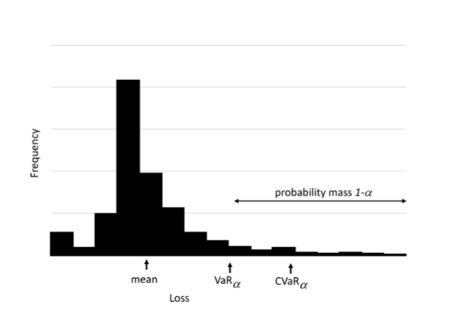
\includegraphics[scale=0.5]{CVaR.jpg}}
    \caption{Relationship between value-at-risk and conditional value-at-risk.}
    \label{fig:CVaR}
\end{figure}

The typical definition of $CVaR_\alpha (X)$ is $CVaR_\alpha (X) = E{X|X > VaR_\alpha (X)}$.
There are alternative ways to define this measure, which are mathematically equivalent.
Rockafellar and Uryasev in~\cite{OptCVaR} (see also~\cite{RemarksCVaR}) defines CVaR as:

\begin{equation}
CVaR_\alpha (X) = \min_u {u + 1/(1-\alpha) E[X-u]^+}
\end{equation}

where $[X-u] = \max (X - u, 0)$. Here, variable $u$ is simply an auxiliary decision
variable whose optimal value turns out to be $CVaR_\alpha (X)$. The above definition
is particularly useful for computation in the context of optimization.

Researchers have argued for using CVaR over VaR as a measure of risk. Theoretically,
CVaR satisfies the assumptions of a so-called coherent risk measure, and VaR does not.
In simpler terms, minimizing VaR is concerned with the numerical value of the 95-th
percentile (say) of the loss, but it does not care about the magnitude of larger losses.
CVaR takes these magnitudes into account.

\subsection{CVaR in Capital Budgeting}
\label{CVaRCapitalBudgeting}
In this section, an explicit risk measure is constructed using a weighted
combination of expectation and CVaR. This approach allows us to parametrically
vary the weight on maximizing expected NPV versus penalizing solutions that yield
low-NPV scenarios, and we denote the weight by $\lambda$ with $0 \le \lambda \le 1$.
Let $NPV(s,\xi)$ denote the net present value under a prioritization decision
specified by decision $s$, and under a realization of the budget and profit of
each project, denoted by $\xi$. Then we seek to solve the following optimization
model:

\begin{equation}
\max_{s\in S} (1-\lambda)E[NPV(s, \xi)] - \lambda CVaR_\alpha [-NPV(s, \xi)]
\end{equation}

When $\lambda = 0$ the model reduces to stochastic optimization model as
discussed in Section~\ref{sec:StochasticCapitalBudgeting}; i.e., we seek
a prioritization decision, $s$, to maximize expected NPV, where ``$s \in S$''
simply indicates the constraints that a prioritized solution must satisfy.
$CVaR_\alpha [X]$ is typically applied to a random variable, $X$, which
represents a loss; i.e., we seek to avoid large values of $X$. In this
context, let $VaR_\alpha [X]$ denote the $\alpha$-level quantile of $X$.
Thus, if $\alpha = 0.75$ then $VaR_0.75 [X]$ is the value such that $75\%$
of the realizations of $X$ have lower values of loss. Suppose for simplicity
that $NPV(s, \xi)$ values are positive. Large values of $NPV(s, \xi)$ are
good, and hence large values of $-NPV(s, \xi)$ (i.e., those closer to zero)
are bad. Using the definition of $CVaR_\alpha [X] = E[X|X > VaR_\alpha [X]]$
we thus have that the conditional value-at-risk is the expected value of loss,
given that the loss exceeds a certain percentile. So, when $\lambda = 1$ we
seek to minimize the expected value of NPV given that they fall below a
threshold. More generally, values of $\lambda$ between 0 and 1 seek a trade-off
between reward and risk, captured by expected NPV and CVaR, respectively.

The full mathematical optimization model of CVaR for capital budgeting problem
is as follows:

\begin{subequations}\label{fullCVaR}
\begin{eqnarray}
& & \max_{x, y, \nu, u} (1-\lambda) \sum _{ \omega  \in  \Omega }^{}q^{ \omega } \sum _{i \in I}^{} \sum _{j \in J_{i}}^{}a_{ij}^{ \omega }x_{ij}^{ \omega } - \lambda[u+1/(1-\alpha)\sum_{\omega \in \Omega} q^\omega \nu^\omega] \\
& & \nu^\omega \ge - \sum _{i \in I}^{} \sum _{j \in J_{i}}^{}a_{ij}^{ \omega }x_{ij}^{ \omega } - u, \omega \in \Omega \\
& & y_{ii^{'}}+y_{i^{'}i} \geq 1,~ i<i^{'}\text{, i, }i^{'} \in I \\
& & \sum_{j=1}^{J_i} x_{ij}^\omega \geq \sum_{j=1}^{J_i} x_{i'j}^\omega + y_{ii'} -1,~ i \neq i^{'}\text{, i, }i^{'} \in I,  \omega  \in  \Omega \\
& & \sum _{i \in I}^{} \sum _{j \in J_{i}}^{}\text{~ c}_{ijkt}^{ \omega }x_{ij}^{ \omega }~  \leq  b_{kt}^{ \omega },~ k \in K, t \in T,  \omega  \in  \Omega \\
& & \sum_{j\in J_i} x_{ij}^{ \omega } \leq 1,~ i \in I, \omega  \in  \Omega \\
& & y_{ii'}, x_{ij}^\omega \in {0, 1} \\
& & \nu^\omega \ge 0, \omega \in \Omega
\end{eqnarray}
\end{subequations}

\subsection{LOGOS Settings for CVaR Problems}
\label{subsec:CVaRSettings}
CVaR approach is an extension for stochastic optimization approach discussed in
Section~\ref{sec:StochasticCapitalBudgeting}. Both of them share the same input
structures except the \xmlNode{Settings} block. In both cases, the user need to
specify a collection of scenarios via \xmlNode{Uncertainties} block. The
\xmlNode{problem\_type} within \xmlNode{Settings} block is used to select the
type of CVaR problems. The currently available CVaR problem types are:
\xmlString{cvarskp}, \xmlString{cvarmkp}, and \xmlString{cvarmckp}. The user can
use \xmlNode{risk\_aversion} (i.e. $\lambda$) and \xmlNode{confidence\_level}
(i.e., $\alpha$) to control CVaR problem.

Example LOGOS input XML for CVaR:
\begin{lstlisting}[style=XML]
<Settings>
<Logos>
  <solver>cbc</solver>
  <solverOptions>
    <StochSolver>EF</StochSolver>
    <risk_aversion>0.1</risk_aversion>
    <confidence_level>0.95</confidence_level>
  </solverOptions>
  <sense>maximize</sense>
  <problem_type>cvarskp</problem_type>
</Settings>
</Logos>
\end{lstlisting}


\subsection{CVaR for Single Knapsack Problem}
\label{subsec:CVaR_SKP}

\vst \noi {\em Model Formulation:}
\begin{subequations}\label{CVaRSimpleKP}
\begin{eqnarray}
& & \max_{x, y, \nu, u} (1-\lambda)  \sum _{ \omega  \in  \Omega }^{}q^{ \omega } \sum _{i \in I}^{} a_{i}^{ \omega }x_{i}^{ \omega } - \lambda[u+1/(1-\alpha)\sum_{\omega \in \Omega} q^\omega \nu^\omega] \\
& & \nu^\omega \ge - \sum _{i \in I}^{} a_{i}^{ \omega }x_{i}^{ \omega } - u, \omega \in \Omega \\
& & \sum_{i \in I} c_{i}^\omega x_{i}^\omega \leq b^\omega, \omega \in \Omega\\
& & y_{ii'} + y_{i'i} \geq 1, i<i'  \\
& & x_{i}^\omega \geq x_{i'}^\omega + y_{ii'}-1, i\neq i' \\
& & x_{i}^\omega, y_{ii'}^\omega \in {0, 1} \\
& & \nu^\omega \ge 0, \omega \in \Omega, \lambda \in [0, 1]
\end{eqnarray}
\end{subequations}

See next section~\ref{subsec:CVaR_DKP} for the example of LOGOS input file, since multi-dimensional Knapsack problem
is just a simple extension of a single-dimensional Knapsack problem, and both of them belong to the same
\xmlNode{problem\_type}: \xmlString{cvarskp}.


\subsection{CVaR for Multi-Dimensional Knapsack Problem}
\label{subsec:CVaR_DKP}

\vst \noi {\em Model Formulation:}
\begin{subequations}\label{CVaRMultiDKP}
\begin{eqnarray}
& & \max_{x, y, \nu, u} (1-\lambda)  \sum _{ \omega  \in  \Omega }^{}q^{ \omega } \sum _{i \in I}^{} a_{i}^{ \omega }x_{i}^{ \omega } - \lambda[u+1/(1-\alpha)\sum_{\omega \in \Omega} q^\omega \nu^\omega] \\
& & \nu^\omega \ge - \sum _{i \in I}^{} a_{i}^{ \omega }x_{i}^{ \omega } - u, \omega \in \Omega \\
& & \sum_{i \in I} c_{it}^\omega x_{i}^\omega \leq b_{t}^\omega, t\in T \\
& & y_{ii'} + y_{i'i} \geq 1, i<i'  \\
& & x_{i}^\omega \geq x_{i'}^\omega + y_{ii'}-1, i\neq i' \\
& & x_{i}^\omega, y_{ii'}^\omega \in {0, 1} \\
& & \nu^\omega \ge 0, \omega \in \Omega, \lambda \in [0, 1]
\end{eqnarray}
\end{subequations}

Example LOGOS input XML:
\begin{lstlisting}[style=XML]
<Logos>
  <Sets>
    <investments>
      1,2,3,4,5,6,7,8,9,10,11,12,13,14,15,16
    </investments>
    <time_periods>
      1,2,3,4,5
    </time_periods>
  </Sets>

  <Parameters>
    <net_present_values index="investments">
      2.315,0.824,22.459,60.589,0.667,5.173,4.003,0.582,0.122,
      -2.870,-0.102,-0.278,-0.322,-3.996,-0.246,-20.155
    </net_present_values>
    <costs index="investments, time_periods">
      0.219,0.257,0.085,0.0,0.0,
      0.0,0.0,0.122,0.103,0.013,
      5.044,1.839,0.0,0.0,0.0,
      6.74,6.134,10.442,0.0,0.0,
      0.425,0.0,0.0,0.0,0.0,
      2.125,2.122,0.0,0.0,0.0,
      2.387,0.19,0.012,2.383,0.192,
      0.0,0.95,0.0,0.0,0.0,
      0.03,0.03,0.688,0.0,0.0,
      0,0.2,0.763,0.739,2.539,
      0.081,0.032,0,0,0,
      0.3,0,0,0,0,
      0.347,0,0,0,0,
      4.025,0.297,0,0,0,
      0.095,0.095,0.095,0,0,
      5.487,5.664,0.5,6.803,6.778
    </costs>
    <available_capitals index="time_periods">
      18,18,18,18,18
    </available_capitals>
  </Parameters>

  <Uncertainties>
    <available_capitals>
      <totalScenarios>10</totalScenarios>
      <probabilities>
        0.012, 0.019, 0.032, 0.052, 0.086, 0.142, 0.235, 0.188, 0.141, 0.093
      </probabilities>
      <scenarios>
        11, 11, 11, 11, 11,
        12, 12, 12, 12, 12,
        13, 13, 13, 13, 13,
        14, 14, 14, 14, 14,
        15, 15, 15, 15, 15,
        16, 16, 16, 16, 16,
        17, 17, 17, 17, 17,
        18, 18, 18, 18, 18,
        19, 19, 19, 19, 19,
        20, 20, 20, 20, 20
      </scenarios>
    </available_capitals>
  </Uncertainties>

  <Settings>
    <mandatory>10,11,12,13,14,15,16</mandatory>
    <solver>cbc</solver>
    <solverOptions>
      <StochSolver>EF</StochSolver>
      <!-- lambda for risk aversion -->
      <risk_aversion>0.1</risk_aversion>
      <!-- confidence level -->
      <confidence_level>0.95</confidence_level>
    </solverOptions>
    <sense>maximize</sense>
    <problem_type>cvarskp</problem_type>
  </Settings>
</Logos>
\end{lstlisting}


\subsection{CVaR for Multiple Knapsack Problem}
\label{subsec:CVaR_MKP}

\vst \noi {\em Model Formulation:}
\begin{subequations}\label{CVaRMKP}
\begin{eqnarray}
& & \max_{x, y, \nu, u} (1-\lambda)  \sum _{ \omega  \in  \Omega }^{}q^{ \omega } \sum_{m\in M} \sum _{i \in I}^{} a_{i}^{ \omega }x_{i, m}^{ \omega } - \lambda[u+1/(1-\alpha)\sum_{\omega \in \Omega} q^\omega \nu^\omega] \\
& & \nu^\omega \ge - \sum_{m\in M} \sum _{i \in I}^{} a_{i}^{ \omega }x_{i, m}^{ \omega } - u, \omega \in \Omega \\
& & \sum _{i \in I}^{} c_{i}^{ \omega }x_{im}^{ \omega }~  \leq  b_{m}^{ \omega },~ m \in M,  \omega  \in  \Omega \\
& & y_{ii'} + y_{i'i} \geq 1, i<i'  \\
& & \sum_{m=1}^{M} x_{im}^\omega \geq \sum_{m=1}^{M} x_{i'm}^\omega + y_{ii'} -1,~ i \neq i^{'}\text{, i, }i^{'} \in I,  \omega  \in  \Omega \\
& & \sum_{m=1}^{M} x_{im}^\omega \leq 1 \\
& & x_{im}^\omega, y_{ii'}^\omega \in {0, 1} \\
& & \nu^\omega \ge 0, \omega \in \Omega, \lambda \in [0, 1]
\end{eqnarray}
\end{subequations}

Example LOGOS input XML:
\begin{lstlisting}[style=XML]
<Logos>
  <Sets>
    <investments>
      1,2,3,4,5,6,7,8,9,10
    </investments>
    <capitals>
      unit_1, unit_2
    </capitals>
  </Sets>

  <Parameters>
    <net_present_values index="investments">
      78, 35, 89, 36, 94, 75, 74, 79, 80, 16
    </net_present_values>
    <costs index="investments">
      18, 9, 23, 20, 59, 61, 70, 75, 76, 30
    </costs>
    <available_capitals index="capitals">
      103, 156
    </available_capitals>
  </Parameters>

  <Uncertainties>
    <available_capitals>
      <totalScenarios>10</totalScenarios>
      <probabilities>
        0.1 0.1 0.1 0.1 0.1 0.1 0.1 0.1 0.1 0.1
      </probabilities>
      <scenarios>
        101, 154,
        102, 155,
        103, 156,
        104, 157,
        105, 158,
        106, 159,
        107, 160,
        108, 161,
        109, 162,
        110, 163
      </scenarios>
    </available_capitals>
  </Uncertainties>

  <Settings>
    <solver>cbc</solver>
    <solverOptions>
      <StochSolver>EF</StochSolver>
      <risk_aversion>1.0</risk_aversion>
      <confidence_level>0.95</confidence_level>
    </solverOptions>
    <sense>maximize</sense>
    <problem_type>cvarmkp</problem_type>
  </Settings>
</Logos>
\end{lstlisting}


\subsection{CVaR for Multiple-Choice Knapsack Problem}
\label{subsec:CVaR_MCKP}

\vst \noi {\em Model Formulation:}
\begin{subequations}\label{CVaRMCKP}
\begin{eqnarray}
& & \max_{x, y, \nu, u} (1-\lambda)  \sum _{ \omega  \in  \Omega }^{}q^{ \omega } \sum_{j\in J_i} \sum _{i \in I}^{} a_{ij}^{ \omega }x_{ij}^{ \omega } - \lambda[u+1/(1-\alpha)\sum_{\omega \in \Omega} q^\omega \nu^\omega] \\
& & \nu^\omega \ge - \sum_{j\in J_i} \sum _{i \in I}^{} a_{ij}^{ \omega }x_{ij}^{ \omega } - u, \omega \in \Omega \\
& & \sum _{i \in I}^{} \sum _{j \in J_{i}}^{}\text{~ c}_{ijkt}^{ \omega }x_{ij}^{ \omega }~  \leq  b_{kt}^{ \omega },~ k \in K, t \in T,  \omega  \in  \Omega \\
& & y_{ii'} + y_{i'i} \geq 1, i<i'  \\
& & \sum_{j=1}^{J_i - 1} x_{ij}^\omega \geq \sum_{j=1}^{J_i - 1} x_{i'j}^\omega + y_{ii'} -1,~ i \neq i^{'}\text{, i, }i^{'} \in I,  \omega  \in  \Omega, and i \neq i' \\
& & \sum_{j=1}^{J_i} x_{ij}^\omega = 1 \\
& & x_{i,j}^\omega, y_{ii'}^\omega \in {0, 1} \\
& & \nu^\omega \ge 0, \omega \in \Omega, \lambda \in [0, 1]
\end{eqnarray}
\end{subequations}

Example LOGOS input XML:
\begin{lstlisting}[style=XML]
<Logos>
  <Sets>
    <investments>
      1, 2, 3, 4, 5, 6, 7, 8, 9, 10, 11, 12, 13, 14, 15, 16, 17
    </investments>
    <options index='investments'>
      1;
      1;
      1;
      1,2,3;
      1,2,3,4;
      1,2,3,4,5,6,7;
      1;
      1;
      1;
      1;
      1;
      1;
      1;
      1;
      1;
      1;
      1
    </options>
  </Sets>

  <Parameters>
    <net_present_values index='options'>
      2.046
      2.679
      2.489
      2.61
      2.313
      1.02
      3.013
      2.55
      3.351
      3.423
      3.781
      2.525
      2.169
      2.267
      2.747
      4.309
      6.452
      2.849
      7.945
      2.538
      1.761
      3.002
      3.449
      2.865
      3.999
      2.283
      0.9
      8.608
    </net_present_values>
    <costs index='options'>
      36538462
      83849038
      4615385
      2788461538
      2692307692
      5480769231
      1634615385
      2981730768
      7211538462
      9038461538
      649038462
      650000000
      216346154
      212500000
      3076923077
      3942307692
      1144230769
      675721154
      1442307692
      99711538
      4807692
      123076923
      138461538
      86538462
      108653846
      75092404
      6413462
      147932692
    </costs>
    <available_capitals>
      15E9
    </available_capitals>
  </Parameters>

  <Uncertainties>
    <available_capitals>
      <totalScenarios>3</totalScenarios>
      <probabilities>
        0.2,0.6,0.2
      </probabilities>
      <scenarios>
        5E9,10E9,15E9
      </scenarios>
    </available_capitals>
  </Uncertainties>

  <Settings>
    <solver>glpk</solver>
    <solverOptions>
      <StochSolver>EF</StochSolver>
      <risk_aversion>0.1</risk_aversion>
      <confidence_level>0.95</confidence_level>
    </solverOptions>
    <sense>maximize</sense>
    <problem_type>cvarmckp</problem_type>
  </Settings>
</Logos>
\end{lstlisting}

    \input{include/rcpsp.tex}
    \section{Plugin for the RAVEN Code}
\label{sec:RavenPlugin}

The deterministic model can be repeatedly solved by changing the input values (i.e.,
\xmlNode{available\_capitals} [$b_{kt}$] and \xmlNode{net\_present\_values} [$a_{ij}$]).
This will allow for what-if sensitivity analysis to identify the
crucial drivers behind the optimal project selection decision. Monte Carlo simulation permits a
powerful variant of this approach in which we model $a_{ij}$ and $b_{kt}$ as random
variables, sample from their distributions, and perform a form of uncertainty quantification
in terms of the resulting distributions governing the binary decisions selected, $x_{ij}$, and
the overall NPV of the selected portfolio.

Example RAVEN input \xmlNode{ExternalModel} XML:
\begin{lstlisting}[style=XML]
<Models>
  <ExternalModel name="singleKnapsack" subType="LOGOS.CapitalInvestmentModel">
    <variables>available_capitals,i1,i2,i3,i4,i5,i6,i7,i8,i9,i10,
      MaxNPV</variables>
    <ModelData>
      <Sets>
        <investments>
          i1,i2,i3,i4,i5,i6,i7,i8,i9,i10
        </investments>
      </Sets>
      <Parameters>
        <net_present_values index="investments">
          18,20,17,19,25,21,27,23,25,24
        </net_present_values>
        <costs index="investments">
          1,3,7,4,8,9,6,10,2,5
        </costs>
        <available_capitals>
          15
        </available_capitals>
      </Parameters>
      <Settings>
        <solver>glpk</solver>
        <sense>maximize</sense>
      </Settings>
    </ModelData>
  </ExternalModel>
</Models>
\end{lstlisting}

As the name suggests, an external model is an entity that is embedded in the RAVEN
code at run time. This object allows the user to import the LOGOS module that will
be treated as a predefined internal RAVEN object. In other words, the
\textbf{External Model} will be treated by RAVEN as a normal external model.
Check the RAVEN user manual for a more detailed description.
\nb The value for attribute \xmlAttr{subType} should always be \xmlString{LOGOS.CapitalInvestmentModel}.

\xmlNode{variables} specifies a list of variable names that need to match
variables used/defined in the LOGOS model. In the above example, the variable
\xmlString{available\_capitals} is sampled by RAVEN, and its value is used
by LOGOS instead of using the default values specified by \xmlNode{ModelData}.
The decision variables \xmlString{i1,i2,i3,i4,i5,i6,i7,i8,i9,i10} and the
objective variable \xmlString{MaxNPV} are collected from the output of the LOGOS model,
and can be stored in the RAVEN data objects.
The XML node \xmlNode{ModelData} is used to specify the LOGOS optimization problem, which
should be consistent with the LOGOS input XML file.

\subsection{Test Automation}
Automated regression testing is a development methodology generally used
to verify the correctness and performance of software after each modification.
This methodology is integrated directly into GitHub and GitLab for RAVEN and
RAVEN-supported plugins. In this case, testing is performed automatically as part of the
continuous integration system (CIS) process whenever a user commits a change to the
repository. Tests of changes across multiple platforms are executed with each pull
request. Results from each test execution are maintained in an approved records
repository in the CIS database, along with results from the timing executions.

\subsection{Testing System Prerequisites}
The module test system consists of scripts written in Bash shell language
and Python. It may be used on any platform supported by RAVEN (i.e.
Linux, Mac, and Windows). The following conditions must be satisfied for the
module test system to function properly:
\begin{itemize}
  \item RAVEN should be installed and updated. This is because RAVEN is used to
  run the module tests;
  \item The system running the tests must be configured with the software prerequisites
  necessary to build and run RAVEN. These include a Python interpreter, Python
  libraries (h5py, matplotlib, numpy, scipy, and scikit-learn), and development
  tools (C++ compiler, Miniconda package manager for Python, and Git source code control);
  \item RAVEN must be built with the appropriate compiler before it can be used to
  run the tests;
  \item The LOGOS submodule must be initialized and fully updated. Additional prerequisites
  include PYOMO, glpk, and coincbc;
\end{itemize}

\subsection{Test Location and Definition}
LOGOS is a RAVEN-supported plugins and managed by Git. RAVEN plugins afford
an option to associate a workflow or a set of RAVEN external models to RAVEN
without having them included in the RAVEN main repository. The benefits include
modularity, access restriction, and regression testing for compatibility with RAVEN
as it continues to grow. In this case, we are able to treat this repository as
separate, yet still be able to use one from within the other. The main structure
of the LOGOS repository is shown in Figure~\ref{fig:Logos}. The folder \textit{tests} contains the input of
the tests, in addition to the corresponding output (in the gold folder) used for
assurance that the behavior of the code is not changed for new modifications. These
tests can also be collected in subfolders based on their characteristics.

\begin{figure}
    \centering
    \centerline{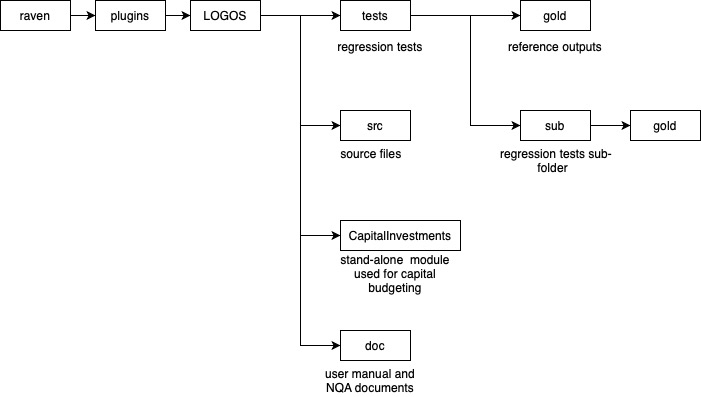
\includegraphics[scale=0.5]{LogosRepo.jpg}}
    \caption{Folder tree of the Logos repository.}
    \label{fig:Logos}
\end{figure}

The RAVEN repository contains a complete testing system for providing regression
testing for itself and its plugins. The LOGOS module tests are defined in the
same manner as for RAVEN. A single test consists of a RAVEN input file
along with associated data needed to perform that run. This can include input data,
external models, and Python files. These may be placed in the \textit{tests} directory
or a related subdirectories. Each directory that contains tests to be run by
the framework must contain a test specification file named “tests”. The syntax of
these files is defined by the RAVEN test framework, which controls how each test
is run and sets the criteria used to determine whether it passed or not. An example
of a test specification file is presented here:
\begin{lstlisting}[language=python]
[Tests]
  [./skp_optimization]
    type = 'RavenFramework'
    input = 'test_skp.xml'
    UnorderedCsv = 'skp/test_skp.csv'
  [../]
[]
\end{lstlisting}
In the above example, one test, named ``skp\_optimization'', is defined using the RAVEN
test module (defined in the test file as “type = `RavenFramework'”). Comparison
criteria are also defined in the “tests” file. In most cases, one or more output
files generated by running the specified input file with RAVEN are compared
against a gold standard provided by the developer and stored in the repository.
Typically, comparisons are performed on numeric values contained in
CSV files up to a defined tolerance. When these file comparisons are specified
by the test developer, reference files must have the same name and be placed
in the gold subdirectory below that containing the “tests” file.

\subsection{Running the Tests}
The integrated tests can be run separately, as indicated by following this pathway:
\begin{lstlisting}[language=bash]
path/to/raven/raven_framework path/to/LOGOS/tests/TestName
\end{lstlisting}

\subsection{Continuous Integration System (CIVET)}
CIVET, developed at INL, is used for continuous integration, verification,
enhancement, and testing of RAVEN and LOGOS. Each time a developer
proposes modification of the contents of the LOGOS repository, CIVET will cause
the automated tests to be run on the modified version. These tests must all pass
before a proposed change can become part of the official repository. In this way,
the LOGOS project is protected from the accidental introduction of flaws into
software that required such a significant investment of resources to develop.

    \section{SSC Cashflow and NPV Models}
\label{sec:SSCNPV}

Imagine a portfolio of candidate projects, in which some of the decisions involve
either replacing an item now or postponing replacement and facing potentially higher
maintenance and replacement costs. We choose to assume that the item must either
be replaced now or in the future, and it is in this context we describe the
appropriate cashflow calculations. We then extend the discussion to allow the
planned replacement to occur in year 2 or 3, for example, rather than in year 1.

We assume that doing nothing is not an option, since the items under consideration
are of significant importance and, if not replaced in due course, would impose
an unacceptable risk to either safety or production.

Notation:

\begin{itemize}
	\item  \( p \) : probability of item failure for one year

	\item  \( C_{P} \) : cost of planned replacement

	\item  \( C_{U} \) : cost of unplanned replacement

	\item  \( C_{D} \) : cost of shutdown per day

	\item  \( D \) : number of days plant is off-line, if a shutdown occurs

	\item  \( N \) : number of years

	\item  \( R \) : discount rate
\end{itemize}


%\begin{comment}
We could incorporate additional parameters, such as weekly or monthly inspection costs,
fixed costs of shutdown in addition to the daily costs specified above, etc. That said,
the setting we describe allows us to illustrate key ideas in the cashflow
calculations for computing NPV.

We further assume that, if we do not replace the item, its failure time is a random
variable that follows a geometric distribution where the probability of failure in
one year is denoted by  \( p \) (i.e., the probability of survival over one year
is  \( 1-p \) ). Thus, if the plant faces a 20-year decision period, the probability
of survival up to year  \( t \) is  \(  \left( 1-p \right) ^{t} \), and the probability
of failing in year  \( t \)  is given by  \( p \left( 1-p \right) ^{t-1} \).

Here is pedantic but useful construct for thinking about the calculations that follow
is to visualize a {\it coin flip}  for each year, yielding a {\it fail}  or {\it no fail}
event for that given year. Immediately after the coin flip, appropriate costs are incurred.
In other words, this discrete view of time with Bernoulli trials is useful to simplify the
logic of the calculations, rather than viewing time as a continuum and teasing
out {\it what happened when} during a given year.

If the item is not replaced today (time  \( t=1 \) ), we can compute the expected
replacement cost in any year  \( t=1, 2, \ldots ,N-1 \)  as:\par

%\begin{comment}


\begin{equation}\label{npv_1}
\mbox{Expected Replacement Cost in Year } t=C_{U}p \left( 1-p \right) ^{t-1}
\end{equation}


Here, we incur this cost only if the coin flips yielded $``$no fail$"$  events in
years  \( t=1, 2, \ldots ,t-1 \), then a $``$fail$"$  event in year  \( t \)
(i.e., we incur the cost through the geometric random variable’s probability mass of having
the first failure in year  \( t \), which is given by  \( p \left( 1-p \right) ^{t-1} \)).

Since we assume the item must be replaced in year  \( N \)  if it has not already failed,
the expected replacement cost does \textit{not} depend on the result of a coin flip
in year  \( N \), in the same way that replacement in year 1 precludes dependence on
the year 1 coin flip. Rather, we incur this cost with certainty in year  \( N \),
as long as the item had not failed in previous years
\(  t=1, 2, \ldots ,N-1 \); In other words, the expected cost is given by:\par

%\begin{comment}

\begin{equation}\label{npv_2}
\mbox{Expected Replacement Cost in Year }N=C_{P} \left( 1-p \right) ^{N-1}
\end{equation}

where the planned replacement cost is used.

In order to illustrate the computation of the cash flows, we further assume that,
if the item is not replaced now, the plant faces a loss of revenue due to a shutdown
at a cost of  \( C_{D} \)  per day. In this case, the expected downtime cost incurred in
year  \( t=1, 2, \ldots ,N-1 \)  is given by:\par

\begin{equation}\label{npv_3}
\mbox{Expected Downtime Cost in Year }t=DC_{D}p \left( 1-p \right) ^{t-1}.
\end{equation}

Again, we assume that the planned replacement in year  \( t=N \)  precludes dependence
on the coin flip and therefore also precludes incurring any downtime cost in that year,
though we acknowledge other assumptions are possible. Thus, for practical purposes,
there is no coin flip in year  \( N. \)

More generally, if the item is not replaced now, the plant will face the possibility
of increased costs due to reliability issues. Such costs include increased
inspection costs, downtime costs for a week-long shutdown, lost revenue from a 6-hour
shutdown, costs associated with the emergency replacement of an item, etc. We can express
the above costs in the following functional form:
\( Re \_ Cost \left( p,t,C_{1},C_{2, \cdots , }C_{M} \right)  \),
where  \( C_{1},C_{2, \cdots, }C_{M} \)  are costs relevant for the considered item, and,
in general,  \( p \)  could be a vector that incorporates multiple types of shutdown. In
our case, the expected downtime cost in year  \( t=1, 2, \ldots ,N \)  is given by a function:
\( Re \_ Cost \left( p,t,C_{P},C_{U},C_{D},D,N \right)  \) , with just a scalar value for  \( p \).

There are two relevant time-series of cash flows: one for replacing the item now and
another for replacing it later, either at failure or at the horizon year  \( N \).
First, consider replacing the item today; in this case, we simply incur the cost of
planned replacement at time  \( t=1 \) (i.e., we incur cost  \( C_{P} \).)

The second time-series of cash flows is for replacing the item in the future.
In this case, for every year  \( t \), we have the expected replacement cost
and downtime cost. So, for any year  \( t=1, 2, \ldots ,N-1 \), the cash
flows will be computed as:\par

\begin{equation}\label{npv_4}
\mbox{Cash Flow Replaced in Year }t= - \left[  \left( C_{U}+DC_{D} \right)  p \left( 1-p \right) ^{t-1} \right]
\end{equation}


and for the final year as:\par

\begin{equation}\label{npv_5}
\mbox{Cash Flow Replaced in Year }N= - \left[ C_{P} \left( 1-p \right) ^{N-1} \right] .
\end{equation}


Note the minus sign in front of the cash flows because all of them are costs
(i.e., cash outflows). The timelines of the two options are illustrated as follows: \par



%%%%%%%%%%%%%%%%%%%% Figure/Image No: 1 starts here %%%%%%%%%%%%%%%%%%%%

\begin{figure}
    \centering
    \centerline{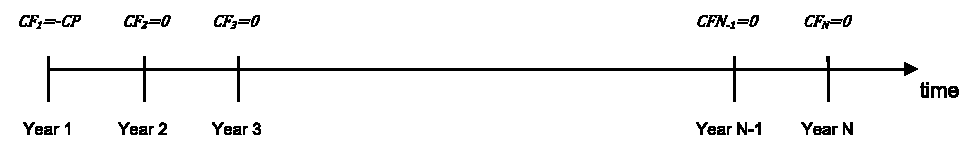
\includegraphics[scale=1]{image1.pdf}}
    \caption{Graphical representation of option 1: replace now.}
    \label{fig:_Graphical_representation_of_option_1_replace_now}
\end{figure}

%%%%%%%%%%%%%%%%%%%% Figure/Image No: 1 Ends here %%%%%%%%%%%%%%%%%%%%


%%%%%%%%%%%%%%%%%%%% Figure/Image No: 2 starts here %%%%%%%%%%%%%%%%%%%%

\begin{figure}
    \centering
    \centerline{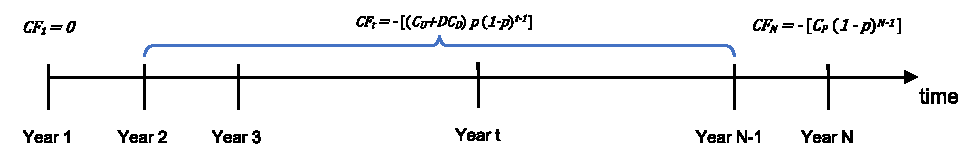
\includegraphics[scale=1]{image2.pdf}}
    \caption{Graphical representation of option 2: replace later.}
    \label{fig:_Graphical_representation_of_option_1_replace_later}
\end{figure}

%%%%%%%%%%%%%%%%%%%% Figure/Image No: 2 Ends here %%%%%%%%%%%%%%%%%%%%


The NPV of option 1 is: \par

\begin{equation}\label{npv_6}
\mbox{NPV option 1}= -C_{P}
\end{equation}

The NPV of option 2 is:\par

\begin{equation}\label{npv_7}
\mbox{NPV option }2= - \left[  \sum _{t=1}^{N-1}\frac{ \left( C_{U}+DC_{D} \right) p \left( 1-p \right) ^{t-1}}{ \left( 1+R \right) ^{t-1}}+\frac{C_{P} \left( 1-p \right) ^{N-1}}{ \left( 1+R \right) ^{N-1}} \right]
\end{equation}


We can compare these options in two ways. The first is to simply compute the
NPV as the difference between the NPV of option 1 and that of option 2 (i.e.,
\( \mbox{NPV}=\mbox{NPV option }1-\mbox{NPV option }2 \)). The resulting equation is:\par

\begin{equation}\label{npv_7}
\mbox{NPV}= -C_{P}+ \left[  \sum _{t=1}^{N-1}\frac{ \left( C_{U}+DC_{D} \right) p \left( 1-p \right) ^{t-1}}{ \left( 1+R \right) ^{t-1}}+\frac{C_{P} \left( 1-p \right) ^{N-1}}{ \left( 1+R \right) ^{N-1}} \right]
\end{equation}


If the project in question is the only one under consideration, and if  \( \text{NPV} \)  $>$ 0,
the decision is to replace the item today; otherwise, we replace it later.
%As we discuss in detail in Section 6, we\ employ an optimization model when multiple projects are considered simultaneously, and we need to stay within annual budgets in terms of, for example, capital costs.  \par

We now extend the above logic to the planned replacement occurring in year \( ~T_{0} \).
We had assumed  \( ~T_{0}=1 \), but now we allow for
delaying this planned replacement to a later year, albeit at the risk of incurring
a failure prior to  \( ~T_{0} \), along with associated unplanned\ replacement
and downtime costs.  If the planned replacement happens at time  \( T_{0} \), the
corresponding time-series of cash flows will become as follows: one for replacing the item
either at failure before  \( T_{0} \)  or at  \( T_{0} \),
and another for replacing it later, either at failure or at the horizon year  \( N \).\par

The first time-series of cash flows is for replacing the item at  \( T_{0} \).
In this case, for every year  \( t=1, 2, \ldots, T_{0}-1 \), we have the expected
replacement cost and downtime cost. So, for any year  \( 1, 2,\ldots, T_{0}-1 \),
the cash flows will be computed as:\par

\begin{equation}\label{npv_8}
\mbox{Cash Flow Replaced in Year }t= - \left[  \left( C_{U}+DC_{D} \right)  p \left( 1-p \right) ^{t-1} \right]
\end{equation}

for  \( t=T_{0} \)  the expected cash flow is:\par

\begin{equation}\label{npv_9}
\text{Cash Flow Replaced in Year }T_{0}= - \left[ C_{P} \left( 1-p \right) ^{T_{0}-1} \right]
\end{equation}

The timeline of this option is illustrated as follows: \par


%%%%%%%%%%%%%%%%%%%% Figure/Image No: 3 starts here %%%%%%%%%%%%%%%%%%%%

\begin{figure}
    \centering
    \centerline{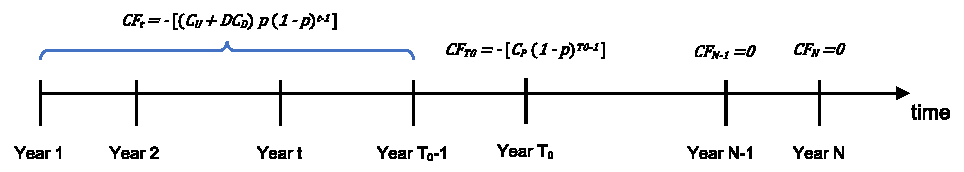
\includegraphics[scale=1]{image3.pdf}}
    \caption{Graphical representation of option 1: planned replacement at $T_0$.}
    \label{fig:_Graphical_representation_of_option_1_planned_replacement_at_}
\end{figure}

%%%%%%%%%%%%%%%%%%%% Figure/Image No: 3 Ends here %%%%%%%%%%%%%%%%%%%%

\begin{equation}\label{npv_10}
\mbox{NPV option }1= - \left[  \sum _{t=1}^{T_{0}-1}\frac{ \left( C_{U}+DC_{D} \right) p \left( 1-p \right) ^{t-1}}{ \left( 1+R \right) ^{t-1}}+\frac{C_{P} \left( 1-p \right) ^{T_{0}-1}}{ \left( 1+R \right) ^{T_{0}-1}} \right]
\end{equation}

Note that, if  \( T_{0}=1 \),  then the first term yields zero, and the NPV of
option 1 reduces to that discussed above (i.e., it equals  \( -C_{P} \).)\par

The second time-series of cash flow is for attempting to delay replacement of
the item to time  \( N \), and incurring the risk of unplanned replacement
and downtime in the meantime. It is the same as we calculated before. \par

\begin{equation}\label{npv_11}
\mbox{NPV option }2= - \left[  \sum _{t=1}^{N-1}\frac{ \left( C_{U}+DC_{D} \right) p \left( 1-p \right) ^{t-1}}{ \left( 1+R \right) ^{t-1}}+\frac{C_{P} \left( 1-p \right) ^{N-1}}{ \left( 1+R \right) ^{N-1}} \right]
\end{equation}

We can compute  \( \text{NPV} \)  as:\par

\begin{eqnarray}\label{npv_12}
\mbox{NPV}&=&\mbox{NPV Option }1-\mbox{NPV Option }2\\
&=& \left[  \sum _{t=T_{0}}^{N-1}\frac{ \left( C_{U}+DC_{D} \right) p \left( 1-p \right) ^{t-1}}{ \left( 1+R \right) ^{t-1}}+\frac{C_{P} \left( 1-p \right) ^{N-1}}{ \left( 1+R \right) ^{N-1}}-\frac{C_{P} \left( 1-p \right) ^{T_{0}-1}}{ \left( 1+R \right) ^{T_{0}-1}} \right]
\end{eqnarray}

A new RAVEN \textbf{External Model} with \xmlAttr{subType} \xmlString{LOGOS.IncrementalNPV}
was created to compute the NPV described above.

Example RAVEN Input \xmlNode{ExternalModel} XML:
\begin{lstlisting}[style=XML]
<ExternalModel name="rvi_model" subType="LOGOS.IncrementalNPV">
  <variables>fp,rvi_npv_a,rvi_npv_b</variables>
  <alias variable="rvi_p_failure" type="input">fp</alias>
  <Cp>19.82</Cp>
  <Cu>39.64</Cu>
  <fp>0.05</fp>
  <Cd>1.</Cd>
  <D>30</D>
  <options>
    <Td>1, 4</Td>
    <output>rvi_npv_a,rvi_npv_b</output>
  </options>
  <discountRate>0.03</discountRate>
  <startTime>2019</startTime>
  <lifetime>20</lifetime>
</ExternalModel>
\end{lstlisting}

In order to use this external model to compute NPV, \xmlString{LOGOS.IncrementalNPV}
should be always used for \xmlAttr{subType}. Except for the common nodes \xmlNode{variables}
and \xmlNode{alias}, this entity accepts the following sub-nodes:
\begin{itemize}
  \item \xmlNode{Cp}, \xmlDesc{float, required parameter}, specifies the cost of planned replacement.
  \item \xmlNode{Cu}, \xmlDesc{float, required parameter}, specifies the cost of unplanned replacement.
  \item \xmlNode{Cd}, \xmlDesc{float, required parameter}, specifies the cost of shutdown per day.
  \item \xmlNode{D}, \xmlDesc{integer, required parameter}, specifies the number of days
  plant is off-line, if a shutdown occurs.
  \item \xmlNode{fp}, \xmlDesc{float, required parameter}, specifies the probability
  of item failure over one year.
  \item \xmlNode{discountRate}, \xmlDesc{float, required parameter}, specifies the discount rate.
  \item \xmlNode{inflation}, \xmlDesc{float, optional parameter}, specifies the inflation rate.
  \default{0.0}
  \item \xmlNode{tax}, \xmlDesc{float, optional parameter}, specifies the tax rate.
  \default{0.0}
  \item \xmlNode{HardSavings}, \xmlDesc{float, optional parameter}, specifies the hard
  savings that would be added to the NPV calculation.
  \default{0.0}
  \item \xmlNode{count}, \xmlDesc{integer, optional parameter}, specifies the number
  of the same items/components that need to be replaced at the same time.
  \default{1.0}
  \item \xmlNode{startTime}, \xmlDesc{integer, required parameter}, specifies the
  start time of project.
  \item \xmlNode{lifetime}, \xmlDesc{integer, required parameter}, specifies the lifetime
  of the project.
  \item \xmlNode{options}, \xmlDesc{optional parameter}, specifies options to compute
  NPVs of planned replacements occurring in different years relative to the start time.
  \begin{itemize}
    \item \xmlNode{Td}, \xmlDesc{comma separated integers, required parameter},
    specifies the lengths of delaying the planned replacement.
    \item \xmlNode{output}, \xmlDesc{comma separated strings, required parameter},
    specifies the output variables corresponding to the different specified lengths of
    delays in \xmlNode{Td}. In order to communicate with RAVEN, these
    variables need to be listed under node \xmlNode{variables}.
    \nb These variables are defined by the user and would be used to store the
    calculated NPVs.
  \end{itemize}
\end{itemize}

The parameters \textbf{Cp, Cu, fp, Cd, inflation, and tax} can be sampled by RAVEN.
If the user specifies these parameters in the input XML \xmlNode{ExternalModel},
the values for these parameters will be replaced by the sampled values from RAVEN.

Example LOGOS Incremental NPV output CSV:
\begin{lstlisting}[language=python]
fp,rvi_npv_a,rvi_npv_b
...
\end{lstlisting}

\nb In order to compute the NPVs, the TEAL plugin is required.
Refer to ~\url{https://github.com/idaholab/raven/wiki/Plugins} for
details on how to access and install the plugins.

The whole calculation flow is depicted in Fig.~\ref{fig:LogosRAVEN}.

%%%%%%%%%%%%%%%%%%%% Figure/Image No: 4 starts here %%%%%%%%%%%%%%%%%%%%

\begin{figure}
    \centering
    \centerline{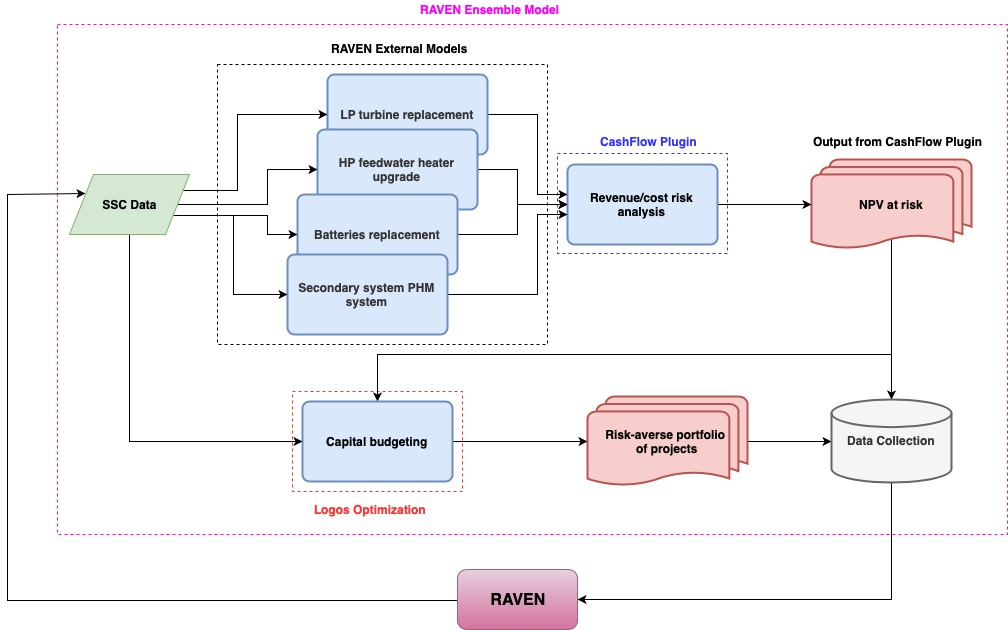
\includegraphics[scale=0.5]{image11.jpg}}
    \caption{Risk-informed capital budgeting via RAVEN and RAVEN plugins.}
    \label{fig:LogosRAVEN}
\end{figure}

%%%%%%%%%%%%%%%%%%%% Figure/Image No: 4 Ends here %%%%%%%%%%%%%%%%%%%%

    \input{include/Knapsack.tex}
    \section{Critical Path Model (CPM)}
\label{sec:CPM}

The CPM model is designed to perform schedule durations calculations provided a set of activities
linked by a graph structure.
This model is designed to be used in a RAVEN workflow where the actitvity duration values can be
changed through a specific sampling strategy (either sampling or optmization).

The schedule requires a ``start'' and an ``end'' activity, a list of additional activities and
their correspoding duration values.
The graph can be imported in two ways. In the first way, the graph is defined in the
\xmlNode{map} nodes. In each instance of the \xmlNode{map} node, an activity is defined and the
following information is required: activity ID (act attribute), activity duration (dur attribute),
and the list of outgoing activities.

Example of CPM input XML in RAVEN input file:
\begin{lstlisting}[style=XML]
  <Models>
    <ExternalModel name="CPMmodel" subType="LOGOS.BaseCPMm odel">
      <variables>start,b,c,d,end,f,g,h,end_time,CP</variables>
      <CPtime>end_time</CPtime>
      <CPid>CP</CPid>
      <map act='start' dur='10'>f,b,h</map>
      <map act='b'     dur='20'>c</map>
      <map act='c'     dur='5' >g,d</map>
      <map act='d'     dur='10'>end</map>
      <map act='f'     dur='15'>g</map>
      <map act='g'     dur='5' >end</map>
      <map act='h'     dur='15'>end</map>
      <map act='end'   dur='20'></map>
    </ExternalModel>
  </Models>
\end{lstlisting}

In the second way, the graph structure can be define in a .py file and it is specified in a
project() class (see below). In this class each activity is define in terms of ID and duration
(see Activity object below).
Then the graph structure is defined through a dictionary, for each activity, a list of list of
outgoing activities is provided.

Example of schedule definition in an external .py file:
\begin{lstlisting}[language=Python]
  from LOGOS.src.CPM.PertMain2 import Pert
  from LOGOS.src.CPM.PertMain2 import Activity

  class project():
    start = Activity("start", 10)
    b     = Activity("b",     20)
    c     = Activity("c",      5)
    d     = Activity("d",     10)
    f     = Activity("f",     15)
    g     = Activity("g",      5)
    h     = Activity("h",     15)
    end   = Activity("end",   20)

    graph = {start: [f,b,h],
             b    : [c],
             c    : [g,d],
             d    : [end],
             f    : [g],
             g    : [end],
             h    : [end],
             end  : []}
  \end{lstlisting}

The CPM model return two parameters. The first one is the critical path time value (i.e., a float),
while the second one is the actual critical path which is represented as a sequence of activity ID
that are part of the critial path (i.e., a string) separated by an underscore.
The RAVEN ID for the critical path time value is specified in the \xmlNode{CPtime}.
The RAVEN ID for the critical path is specified in the \xmlNode{CPid}.




    \section*{Document Version Information}
    This document has been compiled using the following version of the plugin Git repository:
    \newline
    \input{../version.tex}

    % ---------------------------------------------------------------------- %
    % References
    %
    \clearpage
    % If hyperref is included, then \phantomsection is already defined.
    % If not, we need to define it.
    \providecommand*{\phantomsection}{}
    \phantomsection
    \addcontentsline{toc}{section}{References}
    \bibliographystyle{ieeetr}
    \bibliography{user_manual}


    % ---------------------------------------------------------------------- %

\end{document}
